\documentclass[12pt,a4paper,openright,twoside]{report}
\usepackage[english]{babel}
\usepackage[latin1]{inputenc}
\usepackage{fancyhdr}
\usepackage{indentfirst}
\usepackage{graphicx}
\usepackage{newlfont}
\usepackage{amssymb}
\usepackage{amsmath}
\usepackage{latexsym}
\usepackage{amsthm}
\usepackage{booktabs}
\usepackage{array}
\usepackage{braket}
\hyphenation{sil-la-ba-zio-ne pa-ren-te-si}
\pagestyle{fancy}\addtolength{\headwidth}{20pt}
\renewcommand{\chaptermark}[1]{\markboth{\thechapter.\ #1}{}}
\renewcommand{\sectionmark}[1]{\markright{\thesection \ #1}{}}
\rhead[\fancyplain{}{\bfseries\leftmark}]{\fancyplain{}{\bfseries\thepage}}
\cfoot{}
                        

\begin{document}



\begin{titlepage}                      
\thispagestyle{empty}                  
\topmargin=6.5cm                        
\raggedleft                            
\large                                  
\em                                    
Questa \`e la \textsc{Dedica}:\\
ognuno pu\`o scrivere quello che vuole, \\
anche nulla \ldots                      
\newpage                               
\clearpage{\pagestyle{empty}\cleardoublepage}
\end{titlepage}




\pagenumbering{roman}                   
\tableofcontents                       
\rhead[\fancyplain{}{\bfseries\leftmark}]{\fancyplain{}{\bfseries\thepage}}
\lhead[\fancyplain{}{\bfseries\thepage}]{\fancyplain{}{\bfseries INDICE}}

\clearpage{\pagestyle{empty}\cleardoublepage}


\chapter*{Introduction}                 
%%%%%%%%%%%%%%%%%%%%%%%%%%%%%%%%%%%%%%%%%imposta l'intestazione di pagina
\rhead[\fancyplain{}{\bfseries Introduction}]{\fancyplain{}{\bfseries\thepage}}
\lhead[\fancyplain{}{\bfseries\thepage}]{\fancyplain{}{\bfseries Introduction}}
\addcontentsline{toc}{chapter}{Introduction}
Questa \`e l'introduzione.
\clearpage{\pagestyle{empty}\cleardoublepage}

\chapter{Neutrino Physics Overview}                
\rhead[\fancyplain{}{\bfseries Chapter 1: Neutrino Physics Overview}]{\fancyplain{}{\bfseries\thepage}}
\lhead[\fancyplain{}{\bfseries\thepage}]{\fancyplain{}{\bfseries Chapter 1: Neutrino Physics Overview}}
\pagenumbering{arabic}           \label{chapter 1}   
\section{Brief history of neutrinos}
\label{sec:neutrino history}
Neutrinos made their first appearance in modern physics as an hypothesized dark particle proposed by W. Pauli \cite{Pauli} in order to solve the problem introduced by the continuous energy spectrum measured for $\beta$-decay electrons. It was given its name by Enrico Fermi \cite{Fermi}, the first scientist to take in serious consideration Pauli's hypothesis and develop a theory of beta decay that included the new particle as one of the four fermions involved in the correspondent interaction. Fermi's theory led Bethe and Peierls \cite{Bethe-Peierls} to the first estimation of the inverse interaction's cross section:
\begin{equation}
\sigma(\bar{\nu}p\rightarrow ne^+)\leq 10^{-44} \ \text{cm}^2, \ \ E_{\bar{\nu}}\simeq 2 \text{MeV} 
\end{equation}
The smallness of the cross section led the two scientists to conclude that it would be almost impossible to detect such an interaction. \\
Pontecorvo \cite{Pontecorvo} was the first to realize that by using a neutrino flux of about $10^{11}\nu/\text{cm}^2/\text{s}$, of the order of the one produced by an average nuclear reactor, and pointing it towards a ton mass scale detector one could obtain a rate of a few events per day. This idea was put into practice by Reines and Cowan \cite{Reines-Cowan}, whose experiment led to the discovery of the anti-neutrino in 1956. Their technique for the identification of the $\bar nu$ relied on the detection of the light produced by the neutron, in delay with respect to the annihilation of the positron, a template still in use today. \\
In 1962 Lederman, Schwarts and Steinberger \cite{Lederman-Misty-Steinberg} showed the existence of a second type of neutrino, associated with the muon in the main decay mode of the pion: $\pi ^- \rightarrow \mu^-\bar{\nu_\mu} $. This was also the first case in which an accelerator neutrino beam was used in any experiment. Such beam was generated by the decay of pions and other adrons produced in the collision of accelerated protons on a thick shield. A neutrino detector was located behind, revealing the $\mu$'s produced in the $\nu_\mu$ CC interactions.\\
The $\tau$ lepton was discovered at the SLAC accelerator in the seventies, and it would soon be argued that a third neutrino might be associated to it as for the lighter leptons. The study of the decay width of the $Z_0$ produced at LEP \cite{LEP} in $e^+e^-$ collisions excluded any number of SM neutrino families different from three (Fig. \ref{LEPnu-fig}):
\begin{equation}
N_\nu=\frac{\Gamma_{inv}}{\Gamma_{\bar{\nu}\nu}} = 2.984\pm 0.008
\end{equation}
\begin{figure}
	\centering
	\label{LEPnu-fig}
	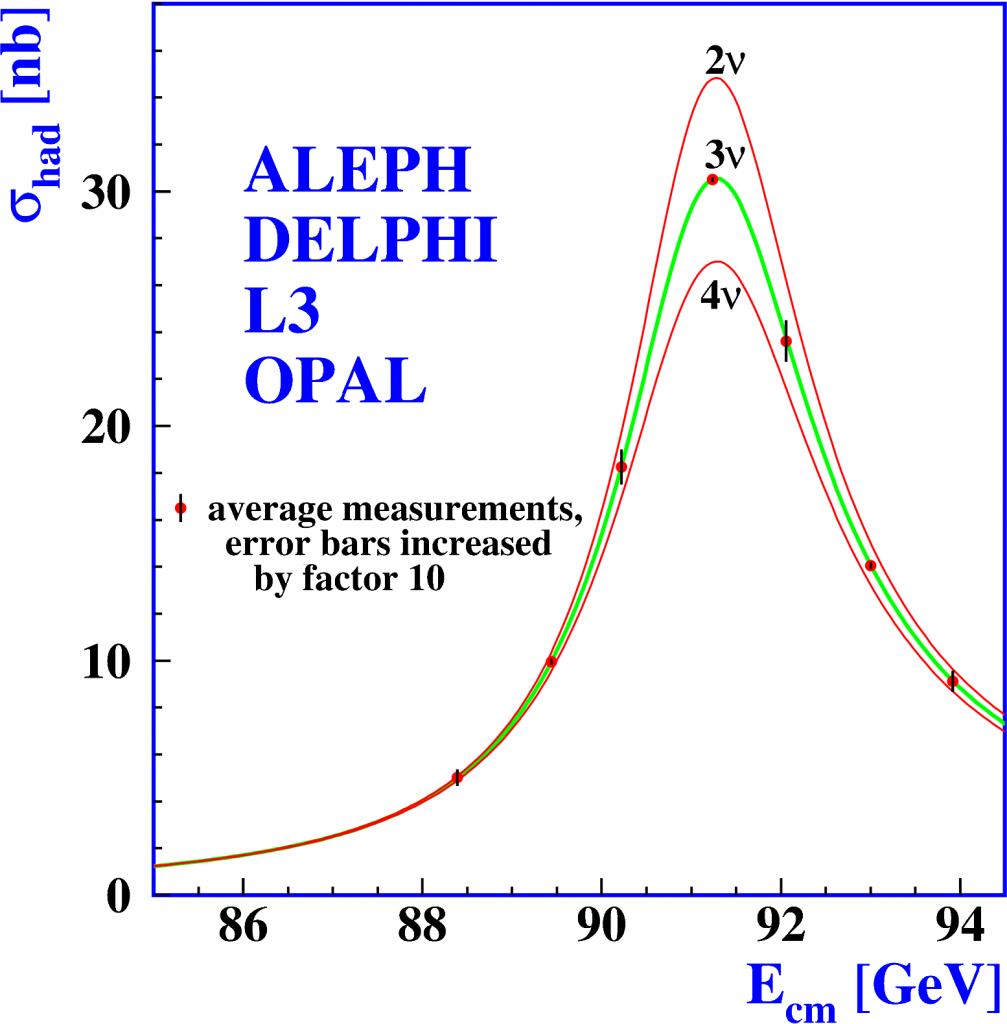
\includegraphics[width=0.5\textwidth]{LEP-NuFlavours.png}
	\caption{Theoretical predictions of the total cross-section for
		the production of hadrons as a function of the center of mass energy for 2, 3 and 4 neutrino families. Experimental data from LEP drawn as dots \cite{LEP}}
\end{figure}
The tau neutrino was finally discovered at Fermilab in 2001 at the DONUT experiment \cite{DONUT} by revealing the taus produced in CC interactions in iron.
\section{Neutrinos in the Standard Model and neutrino masses}
\label{sec:SM}
The Standard Model (SM) of particle physics is a gauge theory defined by the symmetry $SU(3)\times SU(2)_L \times U(1)_Y$ with the subscripts L and Y indicating the left chirality of the particles and their hypercharge respectively. The $SU(3)$ describes the quark interaction in the quark sector while $SU(2)_L \times U(1)_Y$ is related to the electroweak sector. \\
The particles in the SM are divided into bosons of spin 1 that mediate the fundamental interactions (photons for the electromagnetic interactions, $W^ \pm$ and $Z^0$ for the weak sector and 8 gluons for the strong sector), the spin 0 Higgs boson that together with the Higgs field is responsible for the Higgs mechanism and the fundamental fermions quarks and leptons, organized in $SU(2)_L$ left-handed doublets and $U(1)_Y$ right handed singlets (see Table \ref{tab:SM}).

\begin{table}[t]
	\centering
	\setlength{\tabcolsep}{8pt}
	\renewcommand{\arraystretch}{1.3}
	\begin{tabular}{ c c | c c c}
		\hline\hline
		$(1,2)_{-\frac{1}{2}}$ &$(3,2)_{-\frac{1}{6}}$ &$(1,1)_{-1}$ &$(3,1)_{-\frac{2}{3}}$ &$(3,1)_{-\frac{1}{3}}$\\ 
		\hline
		$\begin{pmatrix} \nu_e \\ e \end{pmatrix}_L$ & $\begin{pmatrix} u \\ d \end{pmatrix}_L$ & $e_R$ & $u_R$ & $d_R$\\
		$\begin{pmatrix} \nu_\mu \\ \mu \end{pmatrix}_L$ & $\begin{pmatrix} c \\ s \end{pmatrix}_L$ & $\mu_R$ & $c_R$ & $s_R$\\
	$\begin{pmatrix} \nu_\tau \\ \tau \end{pmatrix}_L$ & $\begin{pmatrix} t \\ b \end{pmatrix}_L$ & $\tau_R$ & $t_R$ & $b_R$\\
		\hline\hline
	\end{tabular}
    \caption{\label{tab:SM}All irreducible fermion representations in the the SM, crouped according to their quantum numbers: $(d_{SU(3)}, d_{SU(2)})_Y$}
\end{table}%
Neutrinos are charge-less fermions that can interact only weakly, either via Neutral Current (NC) interactions mediated via $Z^0$ bosons or charged current via $W^\pm$ bosons. The flavour of the neutrino is simply defined by the charged lepton that is connected to the same charged current vertex:
\begin{equation}
\begin{split}
W^+\rightarrow e^+ + \nu_e\\
   \rightarrow \mu^+ + \nu_\mu\\
   \rightarrow \tau^+ + \nu_\tau
\end{split}
\end{equation}  
In this structure the weak interaction is parity violating and the neutrinos are either left-handed particles $\nu_L$ or right handed anti-particles $\bar \nu_R$. If neutrinos are Dirac fermions, this characteristic makes them massless in the Standard Model, since their mass term, written in its chiral components (Weyl spinors) would be given by :
\begin{equation}
\mathcal{L}^{Dirac}_{mass}=m_D(\bar{\psi}_L\psi_R + \bar{\psi}_R\psi_L), \ \text{with} \ \bar{\psi}_R\psi_L = (\bar{\psi}_L\psi_R)^\dagger 
\end{equation}
It is obvious then that both a left and a right Dirac neutrino would have to exist for the mass term not to be null. This goes in contrast with the observation of neutrino flavour oscillations which that, as we will discuss more in detail later (see Sec. \ref{sec: Oscillation}), are possible only if neutrinos are massive particles.
\\
One strait away solution to this problem is to expand the Standard Model to include a right-handed neutrino $\nu_R$ so that the neutrino and its antiparticle can be described as a 4-state system in a Dirac spinor $\psi=(\psi_L,\psi_R)$, like all the other leptons \cite{Lipari}. The fact that the neutrinos are neutral fermions though, opens up the possibility that they are in fact Majorana particles for which particle and antiparticle are two different spin states of the same particle. Such a fermion would be described by a single Weyl spinor. A Majorana mass term with a single Weyl-spinor, either left or right handed can then be introduced as:
\begin{equation}
\mathcal{L}^{Majorana}_{mass}=- \frac{m_M}{2}[(\psi_L)^Ti\sigma^2\psi_L+h.c.].
\end{equation}
Such a mass term would violate the conservation of the fermionic "charges" by two units, making it plausible only for neutral particles. Since neutrinos have no known charges they can, in principle, both a Dirac and a Majorana term. This could be written as:
\begin{equation}
\mathcal{L}^\nu_{mass}=-\frac{1}{2}(\bar{\psi}_L,\bar{\psi}_L^c) \begin{pmatrix} m_{M,L} & m_D \\ m_D & m_{M,R} \end{pmatrix} \begin{pmatrix} \psi_R^c \\ \psi_R\end{pmatrix}
\end{equation}
where c stands for the the conjugation operation.One can then do some considerations in order to simplify the mixing matrix. The Dirac mass term can be expected to be about the same as for the other fermions in the family and the mass term $m_M,L$ should be small ($m_{M,L}\ll m_D$ ) since it can only be generated by a triplet of Higgs scalars, which is absent from the SM. Finally a right handed neutrino would be completely neutral under the standard-model gauge-group (i.e $sterile$), and it could have a mass above the symmetry breaking scale ($v=$246 GeV), without actually breaking any symmetry. The mass $m_{M,R}$ could then be associated to a different higher mass scale $M$. We then obtain the new matrix:
\begin{equation}
\mathcal{M}\simeq \begin{pmatrix}
0 & m_D \\
m_D & M
\end{pmatrix}
\end{equation} 
This matrix can be diagonalized to obtain two eigenvalues that are approximatly $M$ and $-m_D^2/M$. The two eigenvectors would then be two Majorana particles (per flavour), one very massive and sterile ($m_N\simeq M$) and one very light and weakly interacting ($m_\nu\simeq m_D^2/M$). The second particle would correspond to the neutrinos we normally observe. This so-called $see$-$saw$ mechanism is largely considered to be one of the most natural of the possible explanations for the smallness of the neutrino masses.\\

The main experimental strategy used today if neutrinos are indeed Majorana particles or more canonical Dirac fermions is throgh the observation of the so called neutrinoless double beta decay, a process only possible if neutrinos and antineutrinos are the same particle. Some of the experiments now active in the field now include Gerda, CUORE and CuPID and CANDLES \cite{Petcov}.


\subsection{Limits on neutrino masses}
\label{sec: mass limits}
While the existence of the neutrino oscillation phenomenon is an indicator of the fact that neutrinos must have a mass, as it will be discussed in Section \ref{sec: Oscillation}, they depend only on the squared mass differences between different mass eigenstates and as such, they can't be used to obtain limits on the mass values. A direct measurement of neutrino masses is possible, in principle, using kinematical methods, though these strategies have only produced upper limits so far.\\
For  $\nu_e$ the most effective technique relies on the measurement of the highest kinematically allowed energy in the $\beta$-decay spectrum. Such value is related to the neutrino mass as : $E_{\text{endpoint}}^e\simeq Q -m_\nu$. The best limit is currently set by the KATRIN experiment \cite{KATRIN}, which has recently halved the previous estimates from the Troitsk \cite{Troisk} and Mainz \cite{Mainz} experiments (all study the decay of tritium):

\begin{equation}
\begin{split}
m_{\nu_e} & < 2.05\text{ eV at 95\% c.l. (Troitsk);}\\
          & < 2.3\text{ eV at 95\% c.l. (Mainz);}\\
          & < 1.1\text{ eV at 90\% c.l. (KATRIN);}
\end{split}
\end{equation}
Limits on the masses of the other flavours \cite{PDG} are currently much less stringent and are obtained by studying the pion decay and the $\tau$ decay kinematics for $\nu_\mu$ and $\nu_\tau$ respectively: 
\begin{equation}
\begin{split}
m_{\nu_\mu} & < 170\text{ keV at 90\% c.l. ;}\\
m_{\nu_\tau}& < 18.2\text{ MeV at 95\% c.l. ;}\\
\end{split}
\end{equation}
Limits on the sum of the three masses can also be set by cosmological experiments such as WMAP. These limits are model dependent and in the Standard Cosmological Model are currently set at:
\begin{equation}
\sum_{j}m_j \leq 0.3-1.3 \text{ eV}
\end{equation}
Finally the non observation of double beta decay can set a limit on the electron neutrino effective mass in the case that neutrinos are Majorana particles:
\begin{equation}
\langle m_{\nu_e} \rangle _{eff} \lesssim 0.4 \text{ eV}
\end{equation}

\section{Theory of Neutrino Oscillations }
\label{sec: Oscillation}
If neutrinos have non-vanishing rest mass, the weak and mass eigenstates are not necessarily the same, a fact that is well known in the quark sector where the CKM matrix connects the two types of states. This makes the phenomenon of neutrino oscillations possible i.e. a neutrino produced with a specific flavour can later be measured to have a different flavour. The experimental discovery of this new behaviour in 1998 is today the strongest evidence of the fact that the neutrinos have mass and one of the most powerfull probe into their properties. \cite{Zuber} \cite{Giunti}\\
\subsection{Three flavours oscillations in vacuo}
We start by considering the case where we have 3 orthonormal flavour eigenstates $\ket{\nu_\alpha}$  (where $\alpha = e, \mu, \tau$) which are connected to 3 orthonormal mass eigenstates $\ket{\nu_i}$ via a unitary mixing matrix $U$ \cite{Zuber}:
\begin{equation}
\label{mix:eq}
\ket{\nu_\alpha}=\sum_i U_{\alpha i} \ket{\nu_i} \text{ ;   } \ \ket{\nu_i}=\sum_\alpha U_{\alpha i}^* \ket{\nu_\alpha} \text{ ;  }
\end{equation}
The unitary U matrix, in the case of 3 neutrino flavour and mass eigenstates is the so called PMNS (Pontecorvo-Maki-Nakagawa-Sakata) matrix and can be written as:
\begin{equation}
\begin{split}
U & =
\begin{bmatrix}
1 & 0 & 0 \\
0 & c_{23} & s_{23} \\
0 & -s_{23} & c_{23}
\end{bmatrix}
\quad
\begin{bmatrix}
c_{13} & 0 & s_{13}e^{-i\delta} \\
0 & 1 & 0 \\
-s_{13}e^{i\delta} & 0 & c_{13}
\end{bmatrix}
\quad
\begin{bmatrix}
c_{12} & s_{12} & 0 \\
-s_{12} & c_{12} & 0 \\
0 & 0 & 1
\end{bmatrix} = \\[8pt]
& =
\begin{bmatrix}
c_{12}c_{13} & s_{12}c_{13} & s_{13}e^{-i\delta} \\
-s_{12}-c_{12}s_{23}s_{13}e^{i\delta} & c_{12}c_{23}-s_{12}s_{23}s_{13}e^{i\delta} & s_{23}c_{13} \\
s_{12}s{23}-c_{12}c_{23}s_{13}e^{i\delta} & -c_{12}s_{23}-s_{12}c{23}s_ {13}e^{i\delta} & c_{23}c_{13}
\end{bmatrix}
\end{split}
\end{equation}
%The $(n-1)^2$ independent parameters of the unitary mixing matrix can be conveniently written as: $\frac{1}{2}n(n-1)$ mixing angles of an n-dimentions rotation matrix and $\frac{1}{2} (n-1)(n-2 )$ $CP$-violating phases. \\
\\
where $c_{ij} =\text{cos}\theta_{ij}$, $s_{ij} =\sin\theta_{ij}$, $\theta_{ij}$ are the mixing angles and $\delta$ is the Dirac CP violating phase. In the case of Majorana neutrinos the matrix contains two additional Majorana phases which appear in a diagonal matrix that multiplies U:
\begin{equation}
U_{\alpha \i}^{Majorana}= U_{\alpha i}e^{\lambda_k}
\end{equation} 
These additional phases do not affect neutrino oscillations and cannot be measured in neutrino oscillation experiments, while all the other parameters entering te matrix can be.\\
The mass eigenstates $\ket{\nu_i}$, being the eigenstates of the Hamiltonian ($\mathcal{H}\ket{\nu_i}=E_i\ket{\nu_i}$) show a time dependence :
\begin{equation}
\label{massev:eq}
\ket{\nu_i(t)}=e^{-iE_it}\ket{\nu_i} 
\end{equation} 
with $E_i=\sqrt{\vec{p} \ ^2+m_i^2}$ being the eigenvalues. If we now consider a flavor state $\ket{\nu_\alpha(t)}$ which represents a neutrino of definite flavour created at t=0, from eq. \ref{mix:eq} and \ref{massev:eq} the time evolution of this state is given by:
\begin{equation}
\begin{split}
\ket{\nu_\alpha(t)} & =\sum_i U_{\alpha i}e^{-iE_it}\ket{\nu_k}\\
                    & =\sum_{\beta} \big(\sum_i U_{\alpha i}^* e^{-iE_it} U_{\beta i}\big) \ket{\nu_\beta}
\end{split}
\end{equation}
The superposition of massive neutrino states, which is a pure flavour state at t=0 ($\ket{\nu_\alpha(t=0)}=\ket{\nu_\alpha}$), becomes a superposition of different flavor states at $t>0$. The amplitude of the transition of $\nu_\alpha \rightarrow \nu_\beta$ as a function of time is then:
\begin{equation}
\mathcal{A}_{\nu_\alpha \rightarrow \nu_\beta}(t)= \braket{\nu_\beta|\nu_\alpha(t)}=\sum_i U_{\alpha i}^* U_{\beta k}e^{-iE_it}
\end{equation}
The transition probability is given by the square of the amplitude:
\begin{equation}
P_{\nu_\alpha \rightarrow \nu_\beta}(t)=|\mathcal{A}_{\nu_\alpha \rightarrow \nu_\beta}(t)|^2=
\sum_{i,j}U_{\alpha i}^* U_{\beta i} U_{\alpha j}U^*_{\beta j} e^{-i(E_i-E_j)t}
\end{equation}
In the case that the neutrinos are ultra-relativistic ($v\sim c$) we can approximate:
\begin{equation}
E_i \simeq E + \frac{m_i^2}{2E}; \ \ \ \ t\simeq L;
\end{equation}
with $L$ being the distance between the source and the detector. The probability then becomes:
\begin{equation}
P_{\nu_\alpha \rightarrow \nu_\beta}(L,E)=\sum_{i,j}U_{\alpha i}^* U_{\beta i} U_{\alpha j}U^*_{\beta j} \text{exp} \bigg(-i\frac{\Delta m_{ij}^2L}{2E}\bigg)
\end{equation}
The oscillation probability is then dependent on a set of natural parameters, namely the square difference between the mass eigenstates $\Delta m_{ij}^2=m_i^2-m_j^2$, the three mixing angles $\theta_{ij}$ and the Dirac CP violation phase $\delta$. It also depends on the $L/E$ ratio, which is one of the main features defining the different types of neutrino oscillation experiments (see Sec \ref). It does not however, depend on the absolute mass values  of the eigenstates, making it impossible to determine them in neutrino oscillation experiments. These experiments also do not provide any information about the sign of the square mass differences and are only sensitive to $\Delta m_{23}^2$ and $\Delta m_{13}^2$ which are also commonly referred to as $atmosferic$ and $solar$ mas differences, depending on the type of experiment (Sec. \ref{sec: Oscillation experiments}). Two scenarios consistent with
the experimental measurements are then possible:  the so-called $normal$ and $inverted$ $hierarchy$. In
normal hierarchy, neutrino mass eigenstates are ordered $m_1<m_2<m_3$, while in inverted
hierarchy $m_3<m_1<m_2$ (Fig. \ref{hierarchy:fig}). 
\begin{figure}
	\centering
	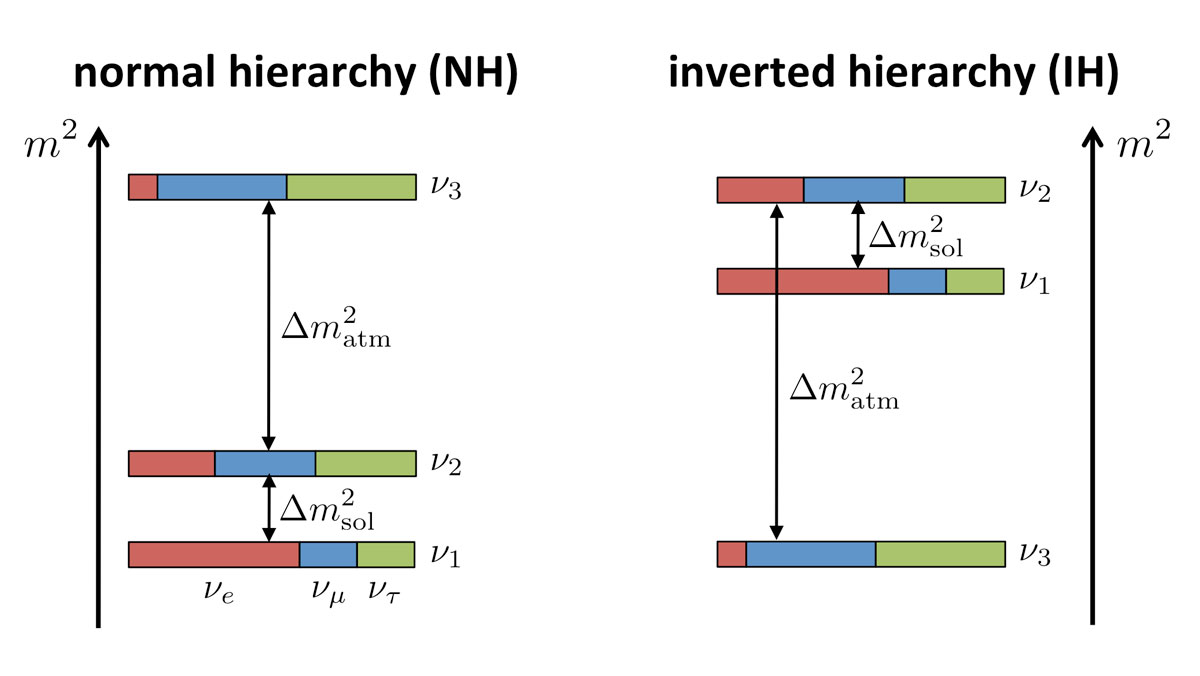
\includegraphics[width=0.8\textwidth]{mass-hierarchy.png}
	\caption{\label{hierarchy:fig}Neutrino mass eigenstates possible orderings in normal (left) and inverted (right) hierarchy. The flavour composition of the three states is shown by dividing the bars into colors: red for $\nu_e$blue for $\nu_\mu$ and green for $\nu_\tau$. \cite{Giunti}}
\end{figure}

\subsection{CP violation}
Knowing from experimental results that all mixing angles are not null, especially $\theta_{13}$, we can see from the mixing matrix, that if the Dirac phase $\delta$ is not null, it can generate CP violation effects in neutrino oscillation. CP violation is manifested if the oscillation probability of $\nu_\alpha \rightarrow \nu_\beta$ are different from the CP conjugate $\bar{\nu}_\alpha \rightarrow \bar{\nu}_\beta$. An observable for such effects would then be the probability asymmetry:
\begin{equation}
\mathcal{A}_{\alpha\beta}^{CP}=P(\nu_\alpha \rightarrow \nu_\beta) - P(\bar{\nu}_\alpha \rightarrow \bar{\nu}_\beta); \ \ \ \ \alpha\neq\beta \ \text{and} \ \alpha,\beta=e,\nu,\tau
\end{equation}
As a consequence of the CPT theorem a CP asymmetry would imply a T asymmetry offering a second observable:
\begin{equation}
\mathcal{A}_{\alpha\beta}^{T}=P(\nu_\alpha \rightarrow \nu_\beta) - P(\nu_\beta \rightarrow \nu_\alpha); \ \ \ \ \alpha\neq\beta \ \text{and} \ \alpha,\beta=e,\nu,\tau
\end{equation}
In the three neutrino mixing case the magnitude of the CP violation is determined by the so-called Jarlskog invariant $J^{CP}_{\alpha\beta}$ in direct analogy with the quark sector:
\begin{equation}
\begin{split}
\mathcal{A}_{\alpha\beta}^{CP}=-16J_{\alpha\beta}^{CP}\sin\bigg(\frac{\Delta m_{12}^2}{4E}L\bigg) \sin\bigg(\frac{\Delta m_{23}^2}{4E}L\bigg) \sin\bigg(\frac{\Delta m_{13}^2}{4E}L\bigg) \\[10pt]
\text{with} \ J_{\alpha\beta}^CP= Im[U_{\alpha1}U_{\alpha2}^*U_{\beta1}^*U_{\beta2}]=\pm c_{12}s_{12}c_{23}s_{23}c_{13}^2s_{13}\sin\delta
\end{split}
\end{equation}
using the same notation as in . The size of CP violation in the neutrino sector is still unknown since the Dirac phase $\delta$ in still unknown. Current data for the mixing angles inply that the value of $J^{CP}_{\alpha\beta}$ should be in the range of:
\begin{equation}
0.026|\sin \delta|\lessapprox |J_{\alpha\beta}^{CP}| \lessapprox 0.036 |\sin \delta|
\end{equation} 
For CP violation effects to be observable both $\sin(\frac{\Delta m_{31}^2L}{2E})$ and $\sin(\frac{\Delta m_{21}^2L}{2E})$ should be large. This is why most future and present experiment that want to perform such measurements are long baseline experiments with $\nu_\mu$ and $\bar{\nu}_\mu$ accelerator beams with energy from $0.7 GeV$ up to a few GeV. 

\subsection{Two flavor scenario}   
An important approximation of the neutrino oscillation phenomenon is the special case in which only two flavours are considered. This casistic is not didactical since it is simpler then the 3-flavour case, but is also useful in data analysis since most experiments are sensible only to the oscillations between two neutrino flavours.\\
In this simplified case the relation between the neutrino states is described by one mixing angle and one mass difference. The unitary transformation then becomes a two-dimensional rotation, analogous to the Cabibbo matrix in the quark sector. In the case of $\nu_e$ and $\nu_\mu$ we get:
\begin{equation}
\begin{pmatrix}
\nu_e \\ 
\nu_\mu
\end{pmatrix}
=
\begin{pmatrix}
\cos\theta & \sin\theta \\ 
-\sin\theta & \cos\theta
\end{pmatrix}
\begin{pmatrix}
\nu_1 \\ 
\nu_2
\end{pmatrix}
\end{equation}
The two-flavour transition probability ,using the formulas from the previous section then becomes:
\begin{equation}
P(\nu_e\rightarrow \nu_\mu) = \sin^22\theta \times \sin^2\bigg( \frac{\Delta m^2L}{4E}\bigg)
\end{equation}
Since no CP violating phase is present his is the same for $P(\nu_\mu\rightarrow \nu_e)$ and for $P(\bar{\nu}_e\rightarrow \bar{\nu}_\mu)$.\\
The $survival$ probability of the particle not changing flavour is simply .
\begin{equation}
P(\nu_e\rightarrow \nu_e)=1-P(\nu_e\rightarrow \nu_\mu)
\end{equation}
The oscillatory term can also be rewritten as:
\begin{equation}
\begin{split}
\sin^2\bigg( \frac{\Delta m^2L}{4E}\bigg)=\sin^2\bigg(\pi \frac{L}{L_0}\bigg) \\[8 pt]
\text{with} \ L_0=4\pi \hbar c\frac{E}{\Delta m^2}
\end{split}
\end{equation}
where $L_0$ is the oscillation length and describes the period of one full oscillation cycle. It is proportional to $E$, and inversely proportional to $\Delta m^2$. The oscillation probability will then be maximum for $L/L_0=1/2$ and its amplitude will be given by $\sin^2\theta$ (Fig. \ref{2oscillation:fig}). 
\begin{figure}
	\centering
	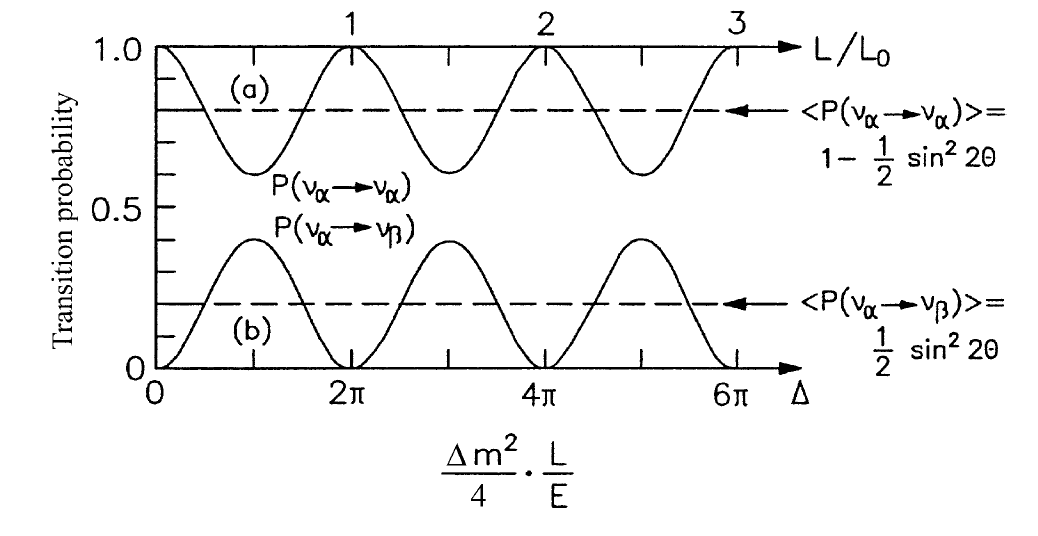
\includegraphics[width=0.7\textwidth]{2flavor_oscillation.png}
	\caption{\label{2oscillation:fig} Two flavor oscillation probability as a functionof $L/L_0$ :disappearene $P(\nu_\alpha\rightarrow \nu_\alpha)$ (up);appearence $P(\nu_\alpha\rightarrow \nu_\beta)$ \cite{Zuber} }
\end{figure}
\subsection{MSW Matter Effects}
\label{sec: matter effects}
When neutrinos travel though dense matter, their propagation can be modified by the coherent forward scattering they experience from particles along their trajectories. The oscillation probability can then become rather different then in vacuum as it was first noticed by Mikhaev, Smirnov and Wolfenstein (MSW), from which the effect takes its name \cite{Wolfenstein}. \\
The MSW effect has origin from the fact that $\nu_e$ and $\bar{\nu}_e$ are the only neutrino flavour that can take part both in charged current interactions, and NC elastic interactions with electrons, while $\nu_\mu$ and $\nu_\tau$ can only have NC interactions with electrons. This introduces and extra potential :
\begin{equation}
V_e= \pm \sqrt{2} G_FN_e
\end{equation} 
where $N_e$ is the electron density in the medium, $G_F$ is the Fermi constant and the sign is positive for neutrinos and negative for antineutrinos.\\
\begin{figure}
	\centering
	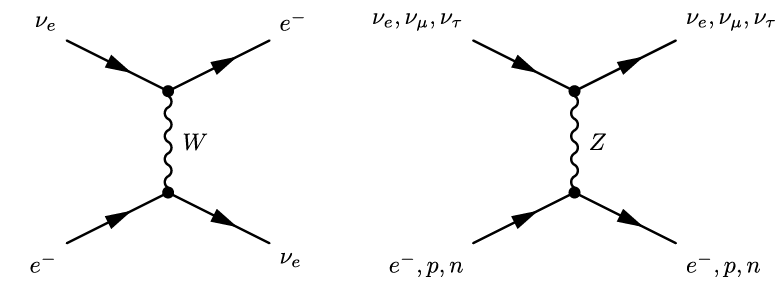
\includegraphics[width=0.7\textwidth]{WZ.png}
	\caption{\label{WZ:fig} Feynmann diagram of CC electronic neutrino interactions $\nu_e+e^- \rightarrow \nu_e+e^-$ (left) and of NC neutrino interactions $\nu_\alpha+e^- \rightarrow \nu_\alpha+e^-$ (right) }
\end{figure}
Using a simplified two flavour approach \cite{Ricciardi} the effective Hamiltonian of neutrino propagation in matter then gains an extra $\nu_e-\nu_e$ element and becomes:
\begin{equation}
\mathcal{H}_M= 
\mathcal{H}+
\begin{pmatrix}
V_e & 0 \\
0 & 0
\end{pmatrix}
=
\bigg(\frac{\Delta m^2}{4E}\bigg)
\begin{pmatrix}
-\cos 2\theta & \sin 2\theta \\
\sin 2 \theta & \cos 2 \theta
\end{pmatrix}
+
\begin{pmatrix}
V_e & 0 \\
0 & 0
\end{pmatrix}
\end{equation}
In the simple case where the matter density is constant, we can then re-diagonalise $\mathcal{H}_M$ to obtain a new mixing matrix and mass eigenstates. We can then denote the new effective parameters as $\theta_M$ and $\Delta m_M^2$ and the oscillation probability takes the usual form:
\begin{equation}
P(\nu_e \rightarrow \nu_\mu)= \sin ^2 2 \theta_M \sin ^2 \bigg(\frac{\Delta m_M^2L}{4E}\bigg)
\end{equation}
The new parameters can be obtain from eq and are:
\begin{equation}
\begin{split}
&\Delta m^2_M =M\Delta m^2\\[8 pt]
&\sin 2\theta_m =\frac{\sin 2\theta}{M}
\end{split}
\end{equation}
with coefficient $M$ being:
\begin{equation}
M=\sqrt{\bigg(\cos 2\theta - \hat{A}\bigg)^2 + \sin^2 2 \theta}
\end{equation}
with:
\begin{equation}
\hat{A}=\pm \frac{2 \sqrt{2}G_FN_eE}{\Delta m^2}
\end{equation}
Matter effects have some very crucial consequences in the field of neutrino oscillation:
\begin{enumerate}
	\item Either long travel distances or high matter densities are necessary in order for the MSW effects to be appreciable (if $\Delta m_M^2L/4E << 1$ we return to vacuum probabilities)
	\item There is a resonant condition for which the oscillation probability is significantly enhanced with respect to the one in vacuum. That is when:
	\begin{equation}
	\hat{A} = \cos 2\theta
	\end{equation} 
	\item Oscillation probabilities can be different for neutrinos and antineutrinos even if there are is no CP violation, due to the $\pm$ sign in the effective potential $V_e$.
	\item The resonant condition can be met only if $\hat{A} > 0$, which depends on the sign of the square mass difference $\Delta m^2$. This fact makes matter effects an effective probe to study mass hierarchy. In particular it can be studied in long baseline accelerator experiments which are sensitive to electron-muon neutrino oscillation ($\Delta m^2 \sim \Delta m_{31}^2$) if $L$ and $E$ are high enough.
\end{enumerate}
\section{Neutrino oscillation experiments}
\label{sec: Oscillation experiments}
The first subdivision between different neutrino oscillation experiments is determined by what the experiment is trying to measure \cite{Giunti}:
\begin{itemize}
	\item \textbf{Appearance experiments}: These experiments look for signals from neutrino flavours that are not present in the initial composition of the flux. The background can be rather small for these experiments, which make them sensitive to small mixing angles.
	\item \textbf{Disappearance experiments}: These experiments measure the number of signals from the various flavours of neutrinos and confront it with the expected one in order to compute the survival probability.
\end{itemize}
The second distinction is then between the different sources of neutrinos then can be used. The most important ones are:
\begin{itemize}
	\item \textbf{Reactor experiments}: they use large fluxes of $\bar{\nu}_e$ produced by beta decays of fission fragments in nuclear power plants; 
	\item \textbf{Accelerator experiments}: they use beams of neutrinos produced in decays of secondary mesons (mainly $\pi$ and $K$) or muons, generated by a proton beam hitting a target. These can be further devided  depending on how the beam is produce. Firstly we have"\textbf{Pion decay in flight}" or \textbf{DIF} beams which are at higher energies and are mainly composed of either $\nu_\mu$ or $\bar{\nu}_\mu$ depending on the polarity of the horn focusing the mesons, with a small percentage of $\nu_e$ from tertiary muon decay. Secondly we have "\textbf{Muon decay at rest}" or \textbf{DAR} which are  in a lower energy range. Finally there are the so called \textbf{Beam dump} or \textbf{prompt} neutrino experiments, in which the proton beam is at very high energy (hundreds of GeVs) and is completely "dumped" in a thick target generating heavy hadrons which equally decay in electron and proton neutrinos;
	\item \textbf{Atmospheric neutrino experiments}: they detect atmospheric neutrinos produced in the atmospheric cosmic ray showers;
	\item \textbf{Solar neutrino experiments}: they detect neutrinos generated in thermonuclear reactions in the centre of the Sun;
\end{itemize}
This distinction is important not only because of the very different experimental setups, but also because the neutrino source and where the detectors are located with respect to it, determine the constants of nature to which the experiments are sensitive. Specifically experiments can be sorted according to  the value of $\Delta m^2$ to which they are sensitive. The condition for an experiment to be sensitive to a specific mass squared difference is that:
\begin{equation}
\frac{\Delta m^2L}{2E}\sim 1
\end{equation}
If this value is too small the oscillation simply does not occur, if it is too large only the average transition probability is measurable and no information on $\Delta m^2$ can be obtained. The different experiments are then classified depending on the ratio $L/E$, which determines the sensitivity:
\begin{itemize}
	\item \textbf{Short Base-Line (SBL)}: These are either reactor or accelerator experiments. In the first case the experiments measure the survival probability and and are active in the $L/E$ range:
	\begin{equation}
	\frac{L}{E}\lesssim 10 \text{m/MeV} \ \ \Longrightarrow \ \ \Delta m^2 \gtrsim 1\text{eV}^2
	\end{equation}
	In the case of  accelerator experiments the range varies depending on the type of beam:
	\begin{equation}
	\begin{split}
	&\frac{L}{E}\lesssim 1 \text{km/GeV} \ \ \ \ \  \Longrightarrow \ \ \Delta m^2 \gtrsim 1\text{eV}^2 \ (DIF)\\ 
	 &\frac{L}{E}\lesssim 1 \text{m/MeV} \ \ \ \ \ \  \Longrightarrow \ \ \Delta m^2 \gtrsim 1\text{eV}^2  \ (DAR)\\
	 &\frac{L}{E}\lesssim 10^{-2} \text{m/MeV} \ \  \Longrightarrow \ \ \Delta m^2  \gtrsim 10^2\text{eV}^2\ (Beam \ dump)
	\end{split}
	\end{equation}
	
	\item \textbf{Long Base-Line (LBN)}: these experiments have sources similar to SBL ones but have a distance between source and detector that is 10 or 100 times larger:
	\begin{equation}
	\begin{split}
	&\frac{L}{E}\lesssim 10^3 \text{km/GeV} \ \ \ \ \  \Longrightarrow \ \ \Delta m^2 \gtrsim 1\text{eV}^2 \ (Accelerator)\\ 
	&\frac{L}{E}\lesssim 10^3 \text{m/MeV} \ \ \ \ \ \  \Longrightarrow \ \ \Delta m^2 \gtrsim 1\text{eV}^2  \ (Reactor)\\
	\end{split}
	\end{equation}
	In this cathegory are also included the Atmospheric neutrino experiments:
	\begin{equation}
	\frac{L}{E}\lesssim 10^4 \text{km/GeV} \ \ \ \ \ \  \Longrightarrow \ \ \Delta m^2 \gtrsim 1\text{eV}^2  \ (ATM)
	\end{equation}
	
	\item \textbf{Very Long Base-Line (VLB)}: these experiments have a distance between source and detector that is 10 or 100 times larger then for  LBN experiments:
	\begin{equation}
	\begin{split}
	&\frac{L}{E}\lesssim 10^5 \text{m/MeV} \ \ \ \ \  \Longrightarrow \ \ \Delta m^2 \gtrsim 10^{-5}\text{eV}^2 \ (Reactor)\\ 
	&\frac{L}{E}\lesssim 10^4 \text{km/GeV} \ \ \ \ \ \  \Longrightarrow \ \ \Delta m^2 \gtrsim 10^{-4}\text{eV}^2  \ (Accelerator)\\
	\end{split}
	\end{equation}
	In this cathegory are also included the Solar neutrino experiments:
	\begin{equation}
	\frac{L}{E}\lesssim 10^{12} \text{m/MeV} \ \ \ \ \ \  \Longrightarrow \ \ \Delta m^2 \gtrsim 10^{-12}\text{eV}^2  \ (Sol)
	\end{equation}
	
\end{itemize}

\subsection{Solar experiments: $\theta_{12}$ and $\Delta m_{12}^2$}
\label{sec: Solar experiments}
\begin{figure}
	\centering
	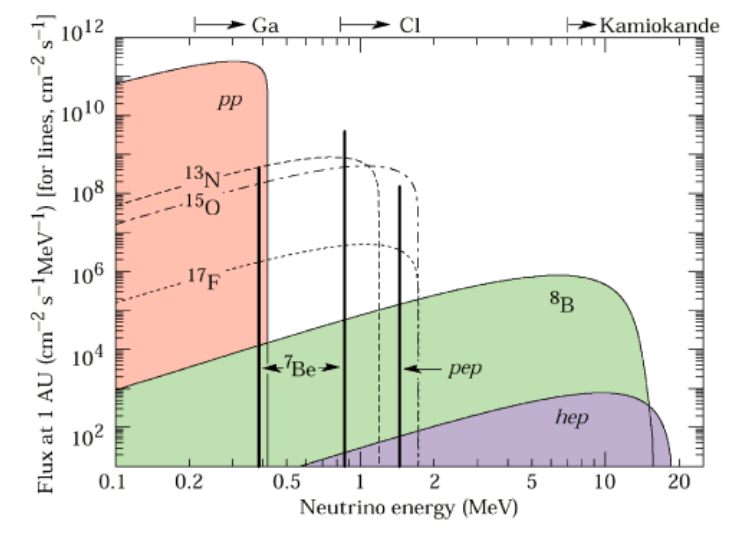
\includegraphics[width=0.6\textwidth]{SSM.png}
	\caption{\label{SSM:fig} Spectrum of solar neutrinos, modelled from the SSM. The arrows indicate the sensitivity range of some of the experiments \cite{Bahcall} }
\end{figure}
The Sun produces an intense flux of neutrinos as a sub-product of some of the thermonuclear reactions that produce energy in its interior by burning hydrogen into helium \cite{Bahcall}. There are two main cycles of  reactions that can produce neutrinos : the pp cycle and CNO (Carbon-Nitrogen-Oxygen) cycle. Both can be summarized as:
\begin{equation}
4p \rightarrow \ ^4He+2 e^- + 2\nu_e
\end{equation}  
The expected flux of $\nu_e$, in the hypothesis that they are massless can be computed using the standard solar model (SSM), which is a detailed simulation of the reactions taking place in the solar interior (Fig. \ref{SSM:fig}).\\
The solar neutrino experiments can be divided into two main categories depending on the revelation techniques: radiochemical and Cherenkov. In the first field we find experiments such as Homestake \cite{Homestake}, Gallex/GNO \cite{Gallex} and Sage \cite{Sage} (using $^37$Cl, $^71$Ga and $71$Ge respectively). These have a relatively low energy threshold ($E_\nu\gtrsim 0.23-0.81$ MeV) for all flavours of neutrinos, but they are not able to give any information on  direction, energy or time of the event.\\
The Cherenkov technique was pioneered by the Kamiokande experiment \cite{SuperK}, consisting of a tank of about 3000 tons of pure water and 1000 photomultipliers positioned on the inner walls. It consisted in observing the Cherenkov light produced by recoil electrons in  elastic scattering interactions of $\nu_e$ with $e^-$, which have a larger threshold of $E\gtrsim 5 \text{MeV}$:
\begin{equation}
\text{(ES)} \ \ \nu_e + e^- \rightarrow \nu_e + e^- \ \ \ \ E\gtrsim 5 \text{MeV}
\end{equation}
\begin{figure}[t]
	\centering
	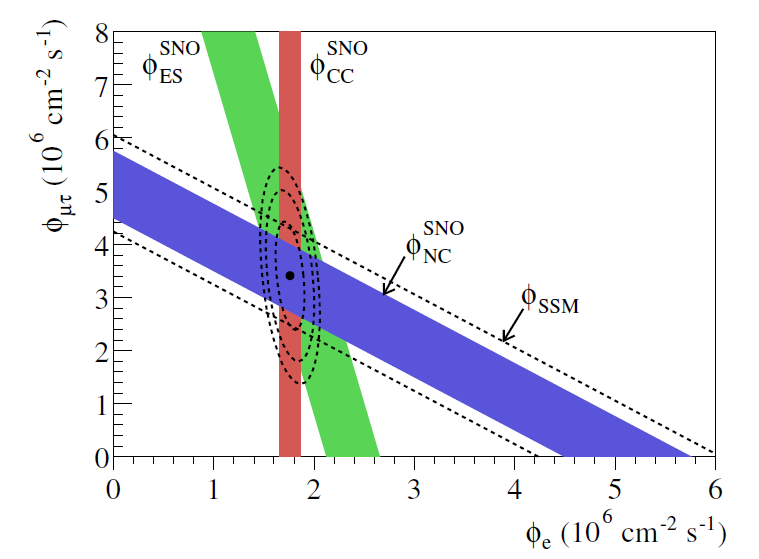
\includegraphics[width=0.7\textwidth]{SNO.png}
	\caption{\label{SNO:fig} Flux of muon and tau neutrinos $\phi_{\mu\tau}$ over electron neutrino $\phi_e$ as measured by SNO. The three coloured bands correspond to the three possible interactions: electron scattering ES (green); charged current CC (red); neutral current NC (blue). The dashed band gives the prediction from the SSM which is in agreement with the NC measurements. \cite{SNO}   }
\end{figure}
This technique was capable of measuring neutrino interactions in real time while also giving informations on direction and energy. This capability was crucial in confirming the existence of the so called \textit{solar neutrino problem}, a deficit in the number of neutrinos arriving from the Sun between 1/2 and 2/3 with respects to the predictions of the SSM, measured by the earlier radiochemical experiments. \\
The Kamiokande experiment was not able to measure both the flux of $\nu_e$ and the combined flux between the three flavors. This was made possible by the SNO experiment \cite{SNO} in which, thanks to the use of heavy water ($d_2O$) rather than purified water as target, two more reactions were available for detection:
\begin{equation}
\begin{split}
\text{(CC)} & \ \ \ \nu_e+d \rightarrow p+p+e^-; \ \ \ E\gtrsim\text{5MeV} \\
\text{(NC)} & \ \ \ \nu_f+d \rightarrow p+n+\nu_f; \ \  f=e,\mu,\tau  \ \ E\gtrsim\text{2.2MeV}
\end{split}
\end{equation}  
Since the first reaction is sensitive only to $\nu_e$ while the second is sensitive to all flavors, one can compare the two rates in order to establish if the solar neutrino flux contains $\nu_\mu$ and $\nu_\tau$ or not and in which measure. What SNO found was that the combined tau and mu fluxes were two
times more intense than the $\nu_e$ one and that the total flux was in agreement with the predictions from the SSM (Fig. \ref{SNO:fig}). \\
The results from solar neutrino experiments can be interpreted as due to flavour oscillation. The characteristic L/E for these experiments are of the VLB range, making them sensitive to the $\Delta m^2_{12}$ mass squared difference and to $\sin2\theta_{12}$. For this reason the two parameters are often referred to as solar mass difference and solar mixing angle ($\Delta m^2_\odot, \theta_\odot$). As already noted these two parameters can be measured also by VLB reactor experiments such as KamLand \cite{kamland} (discussed in Sec.\ref{sec: Reactor experiments}). The most precise values for the parameters are obtained combining the results from both (Fig. \ref{kamland:fig}).\\
Other important and more recent Solar experiments include Borexino \cite{Borexino}, which was the first with an energy threshold low enough to measure the monochromatic flux of $^7Be$ and $pep$ neutrinos and Super-K, the successor of Kamiokande. The results from both experiments are in agreement with the neutrino oscillation hypothesis.

\subsection{Reactor experiments}
\label{sec: Reactor experiments}
\subsubsection{VLB: confermation of solar experiment results}

\begin{figure}
	\centering
	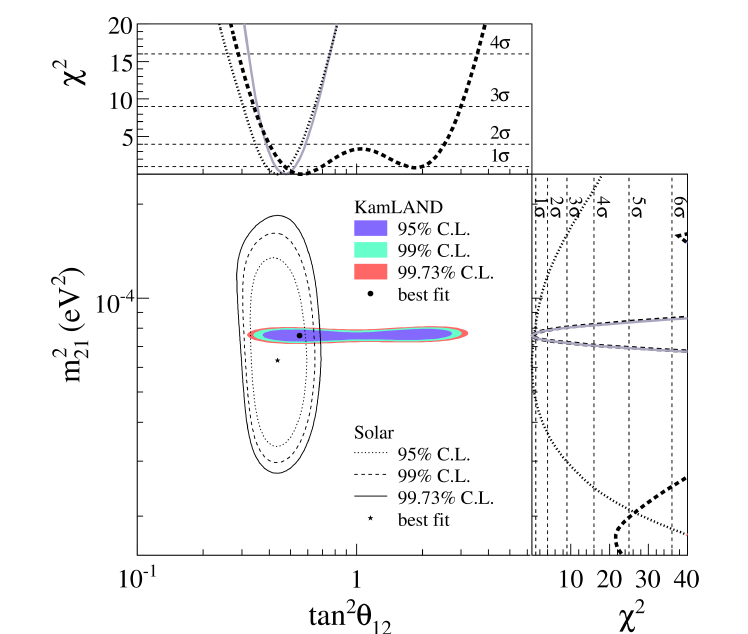
\includegraphics[width=0.7\textwidth]{kamland.png}
	\caption{\label{kamland:fig} Confidence level intervals for the solar oscillation parameters from KamLAND and the combined results from solar experiments. The side-panels show the respective $\chi^2$ profiles: KamLAND (dashed); solar experiments (dotted) individually; combined (solid) \cite{kamland}}
\end{figure}
Neutrinos from nuclear reactors are mostly $\bar{\nu}_e$ with energy of the order of the MeV. This makes the particles above threshold for electronic CC interactions, but not for other flavours, which means that if the neutrino oscillates it cannot be detected anymore. Reactor experiments can then measure the disappearance probability of the $\bar{\nu}_e$ and they are usually sensitive to small values of $\Delta m^2$ due to the low energy spectrum of the neutrinos. \\
Very Long Baseline experiments proved to be sensitive to the solar square mass difference and were able to give confirmation on the Solar experiment results, while at the same time improving the sensitivity to the parameter and beginning the precision era of neutrino physics. \\
In particular the KamLAND experiment, located in the Kamioka mines in Japan , was the first to give independent confirmation of the results from the solar neutrino sector. It consists of a 1000 ton liquid scintillator detector measuring the interactions of $\bar{\nu}_e$ from a cluster of nuclear reactors located  at an average distance of $L \simeq 175$km. The antineutrinos interact via inverse beta decay at an energy threshold of $E>2.6$MeV:
\begin{equation}
\bar{\nu}_e + p \rightarrow e^+ +n \ \ \ \ E>\text{2.7 MeV}
\end{equation}
As mentioned in Section \ref{sec:neutrino history}, this is the same reaction used by Reines and Cowan in their famous experiment and the signature given by the $e^+$ annihilation and the delayed neutron thermalisation and capture proved very effective in the reduction of background. This level of precision was also crucial in excluding alternative explanations for neutrino oscillations based on exotic interactions or magnetic transition moments \cite{Wagner}.

\subsubsection{Measurement of $\theta_{13}$ }
\begin{figure}
	\centering
	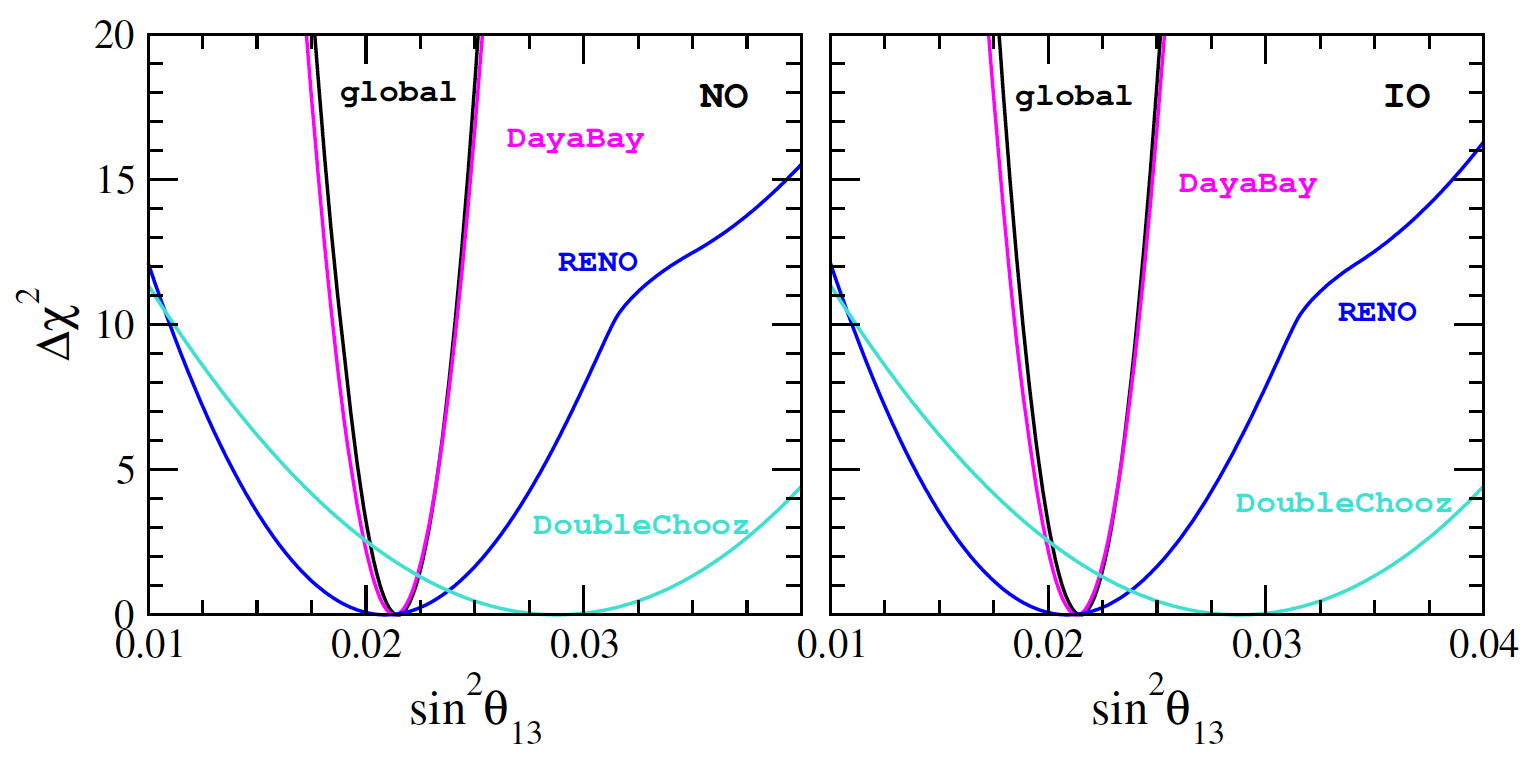
\includegraphics[width=0.8\textwidth]{theta13.png}
	\caption{\label{theta13:fig} $\chi^2$ profile as a function of $\sin\theta_{13}$ for RENO DataBay and Double Chooz and the combined result (black line). The results are fitted for normal ordering (left) and inverse ordering (right) \cite{Farzan-Tortola}}
\end{figure}
Recently Long Baseline experiments such as Data Bay \cite{Data Bay}, RENO \cite{RENO} and Double Chooz \cite{Double Chooz} have been able to measure the disappearance of reactor electron antineutrinos at distances $L\sim$1 km. This is the typical $L/E$ for which oscillations are mainly driven by the mixing angle $\theta_{13}$.\\
Compared to previous experiments such as CHOOZ and Paloverde,  these have not only access to larger statistics, thanks to the increased reactor power and larger detectors,but they also have access to multiple detectors at different distances from the reactor core. Measurements at the closest detectors can then be utilized to more accurately predict the expected number of events at the more distant ones.  \\
The combined results from the experiments are shown in Fig. \ref{theta13:fig}
\subsection{Atmospheric experiments: $\Delta m_{31}^2 $ and $ \theta_{23}$}
\label{sec: atmospheric experiments}
\begin{figure}
	\centering
	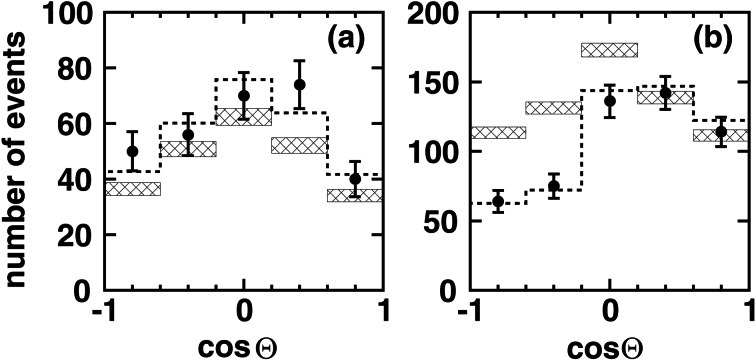
\includegraphics[width=0.9\textwidth]{superk.png}
	\caption{\label{superk:fig} Zenith angle $\Theta $ distributions for the most energetic multi-GeV atmospheric neutrino events measured by Super-Kamiokande over a 535 days period. Filled histograms are the Monte Carlo predictions and dotted histograms are the experimental measurements. Right and left panels are $\mu$-like and e-like events respectively. \cite{Superk atm}}
\end{figure}
\begin{figure}
	\centering
	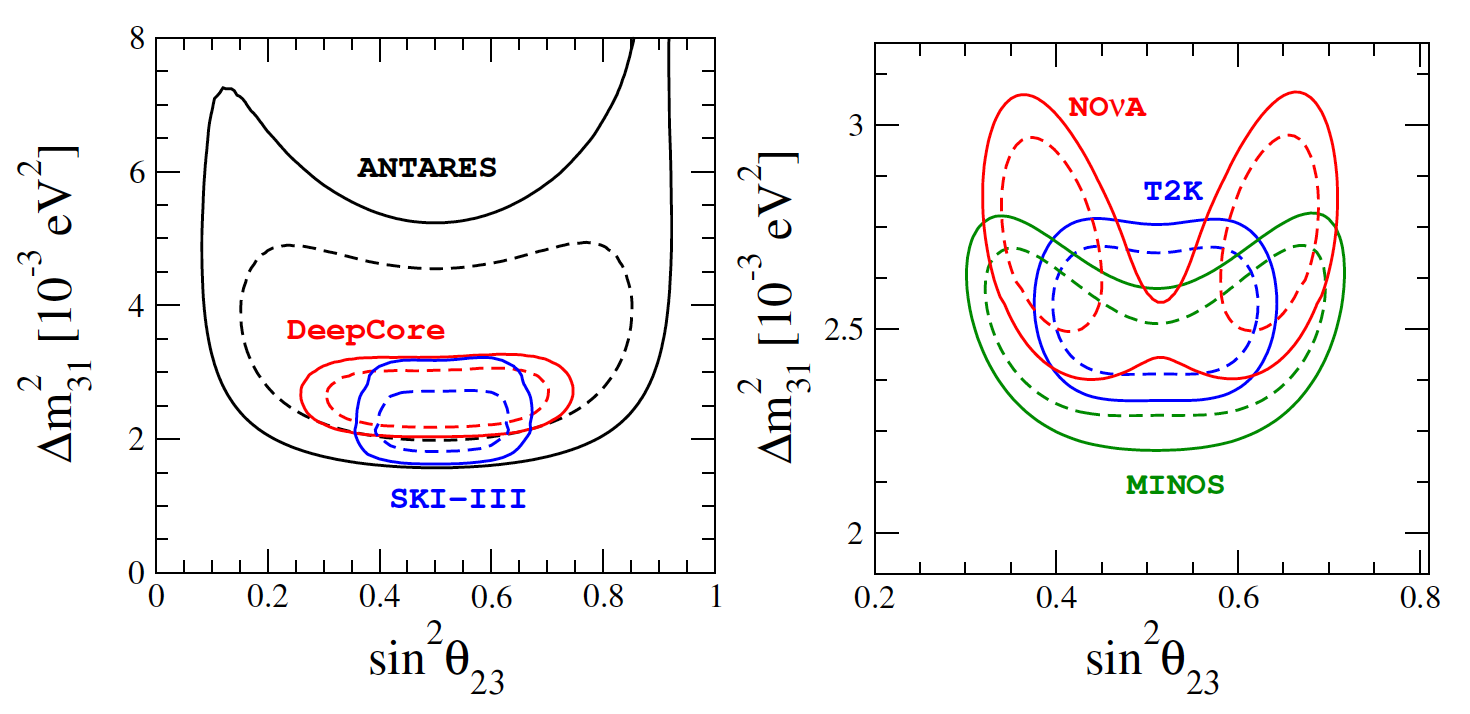
\includegraphics[width=0.9\textwidth]{atmnu.png}
	\caption{\label{atmnu:fig}90\% CL (straight line) and 99\% CL(dashed line) C.L. regions in the atmospheric parameter plane ($\Delta m_{31}^2$ over $sin^2 \theta_{23}$ from atmospheric (left) and long baseline accelerator (right) experiments, assuming normal mass hierarchy. \cite{Farzan-Tortola} }
\end{figure}
The cosmic ray interactions with the atmosphere nitrogen and oxygen nuclei produce mostly pion and kaons that decay in electron and muon neutrino as well as antineutrinos. $\nu_e$ decay from the chain : $\pi \rightarrow \mu \nu_\mu$ followed by $\mu \rightarrow e \nu_\mu \nu_e $. One then would expect the ratio to be of the order:
 \begin{equation}
 R= \frac {N (\nu_\mu + \bar{\nu_\mu})}{N (\nu_e + \bar{\nu_2} )} \sim 2
 \end{equation}
Experiments originally built to look for proton decay in the '70s and '80s, which had atmospheric neutrinos as background, were the first to observe a deficit with respect to the Monte Carlo expectations, measured originally as the ratio : $R_{\mu / e}/ R_{\mu/e}^{MC}$. Two main categories of detectors were in operation: water Cherenkov tanks such as Super Kamiokande \cite{Superk atm} and iron calorimeters such as Soudan2 \cite{soudan 2} and Macro \cite{MACRO}. The first kind of detectors are constituted of tanks filled with water in the order of 1 ton, and they detect the Cherenkov light rings produced by the charged lepton using photo multipliers placed on the inside of the walls. Iron calorimeters are instead constituted of layers of iron, acting as a passive materials and active layers, made for example of plastic drift tubes, which track either the electromagnetic showers produced by $e^\pm$ or long muonic tracks. Both techniques are capable of flavour identification and direction and energy estimation.\\
In 1998 the SuperKamiokande identified the origin of this anomaly to be caused by neutrino oscillation. The experiment distinguished between muon and electron neutrino events, measured the lepton zenith angle with respect to the Earth's axis (correlated to that of the parent neutrino) and divided the samples differentiating between the lepton energy (the more energetic events having a stronger direction dependency with that of the parent neutrino). These measurements made it possible to observe the variation of the flux as a function of the energy and zenith angle and thus the $L/E$ travelled by the parent neutrino (Fig.\ref{superk:fig}).\\
 SuperK showed that while the electron events had no observed reduction, the muon events had a deficit of almost 50\% for up-going neutrinos ($\cos\Theta = -1$). This is explained considering a flavour oscillation dominated by the parameters $\Delta m_{23}^2 \sim \Delta m_{13}^2$ and $\theta_{23}$ that for this reason are often referred to as atmospheric oscillation parameters : $\Delta m_{ATM}^2, \ \theta_{ATM}$. The best fit values for these parameter are today given by combining the results of SuperK with the ones from modern neutrino telescopes ANTARES and IceCube (Fig. \ref{atmnu:fig}). The other possibility is to measure these parameters in Long Baseline accelerator experiments.
\subsection{Accelerator experiments}
\label{sec: accelerator experiments}
As already mentioned in Section \ref{sec: Oscillation experiments}, neutrino beams can be produced in a variety of ways by using protons from particle accelerators. The energy of the primary beam and the distance between the production point and the detector can be selected almost at will. This means that in principle accelerator experiments can be sensitive to most oscillation parameters, depending on the L/E that is chosen at time of construction. \\
As already made clear in section Long baseline accelerator experiments are sensitive to the atmospheric parameters ($\Delta m_{ATM}^2, \theta_{ATM}$). They can measure both appearance and disappearance probability and have usually multiple detector: usually a near detector, which measures the neutrino spectral composition at production and a far detector which is put at a convenient L in order to measure the spectrum again, after oscillation.\\
The first two experiments to confirm the atmospheric oscillation results were K2K (KEK to Kamioka) in Japan and MINOS at Fermilab. K2K used a beam of about 98\% $\nu_\mu$ with a mean energy of about 1.3 GeV produced from 12 GeV protons accelerated at the KEK synchrotron. The experiment had a near detector at about 300 m from the proton target, and used SuperK as its far detector at about 250km. The K2K data sample taken from 1999 to 2005 (K2K-I and II) contained about 112 muonic events versus the 158 expected without oscillation, confirming the findings in the atmospheric sector \cite{k2k}. MINOS also looked for $\nu_\mu$ disappearence using the NuMi neutrino beam at $E\sim3$GeV. Much like K2K it had a near detector at about 1 km from the source and it used an older detector in the Soudan mines at about 735 km away as its far detector. The first results published in 2006, combined with the ones from K2K first confirmed neutrino oscillations at 5$\sigma$ \cite{MINOS}.\\
Long Baseline experiments such as OPERA and ICARUS worked instead in the appearence channel looking for signatures of $\nu_\tau$ in $\nu_\mu$ beams. Opera in particular fount 5 $\nu_\tau$ candidates in a sample of $1.8 \times 10^{19}$ POT (protons on target) from the CNGS beam. This was enough to confirm muon neutrino oscillation at 5$\sigma$ \cite{OPERA}. Short baseline experiments such as NOMAD \cite{Nomad} and CHORUS \cite{Chorus} at CERN also studied the $\nu_\mu \rightarrow \nu_\tau$ channels but did not observe any oscillations. \\
Current experiments such as T2K  (Tokai to Kamioka) \cite{T2K}, the successor of K2K, and NoVa \cite{Nova} both use muon neutrino beam and perform precision measurements in both appearance and disappearance channels. Allowed CL areas for the atmospheric parameters $\Delta m_{31}^2$ and $\sin^2 \theta_{23}$ obtained from T2K, NoVa and MINOS data can are shown in Fig. \ref{atmnu:fig}. DUNE will also be one such experiment as it will be discussed in the next chapter.
\subsection{$\delta_{CP}$ experimental results}
\begin{figure}[t]
	\centering
	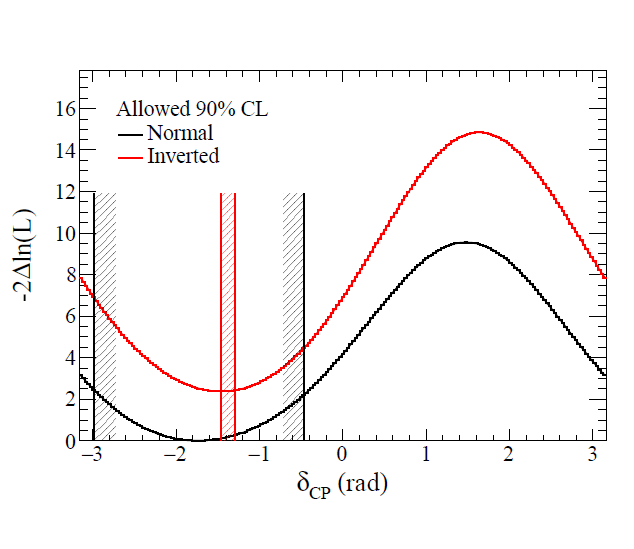
\includegraphics[width=0.48\textwidth]{cpt2k.png}
	\hfill
	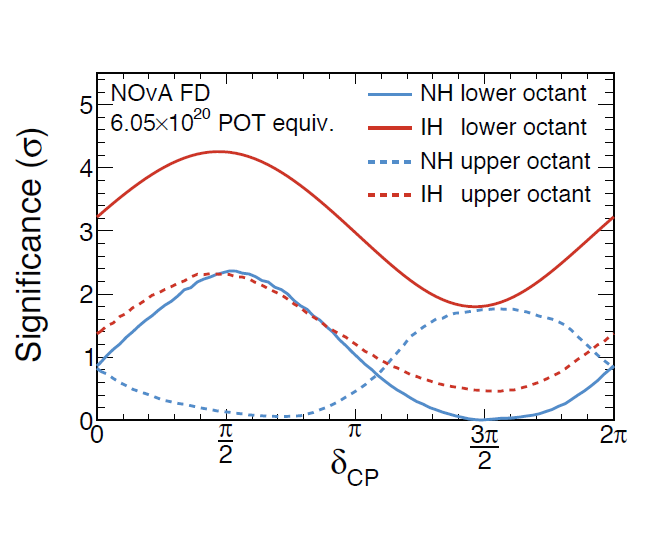
\includegraphics[width=0.48\textwidth]{cpnova.png}
	\caption{\label{cp:fig} (Left) Log-likelihood function of $\delta_CP$ with 90\% CL for normal (black) and inverted (red) hyerarchy at T2K (Right) Significance as function of $\delta_CP$ at NO$\nu$A in all combinations of mass ordering and $\theta_{23}$ octant \cite{t2k deltacp} }
\end{figure}
As already mention in Section most experiments that want to perform  measurements of the CP phase are long baseline experiments with $\nu_\mu$ and $\bar{\nu}_\mu$ accelerator beams with energy from $0.7 GeV$ up to a few GeV. Specifically the CP asymmetries are usually measured as:
\begin{equation}
\mathcal{A}_{CP}=\frac{P(\nu_\mu \rightarrow \nu_e)- P (\bar{\nu}_\mu\rightarrow \bar{\nu}_e)}{P(\nu_\mu \rightarrow \nu_e)+ P (\bar{\nu}_\mu\rightarrow \bar{\nu}_e)}
\end{equation}
This observable can be approximated in the three-flavour case as \cite{deltaCP}:
\begin{equation}
\label{eq:asymmetry}
\mathcal{A}_{CP} \simeq \frac{\cos\theta_{23} \sin2\theta_{12}}{\sin\theta_{23}\sin\theta_{13}}\bigg( \frac{\Delta m_{21}^2 L}{4E_\nu}\bigg)\sin\delta_{CP} + \text{matter effects}
\end{equation}
It is clear then that if $\delta_{CP}$ is different from $0^\circ$ and $\pm 180 ^\circ$ one should expect to observe CP violation in the leptonic sector and $\mathcal{A}_{CP}$ would be different from 0 (i.e. $P(\nu_\mu \rightarrow \nu_e) \neq P(\bar{\nu}_\mu \rightarrow \bar{\nu}_e)$).\\
The latest measurements of $\delta_{CP}$ are from T2K \cite{t2k deltacp}. The experiment measured both the $\nu_\mu$ survival probability and the $\nu_e$ appearance probability and then did the same for $\bar{\nu}_\mu$. The analysis excludes $\delta_{CP}=0^\circ,\pm 180 ^\circ$ at 90\% CL for both mass orderings.\\
Similar measurements have been performed by the NO$\nu$A experiment. The analysis found two best-fit points for normal mass ordering : $\sin^2\theta_{23}= 0.404$ $\delta_{CP}=1.48\pi$ and $\sin^2\theta_{23}= 0.623$ $\delta_{CP}=0.74\pi$. It also found that the inverted mass ordering is disfavoured at $>93\%$ regardless of the value of the CP phase.
\begin{figure}
	\centering
	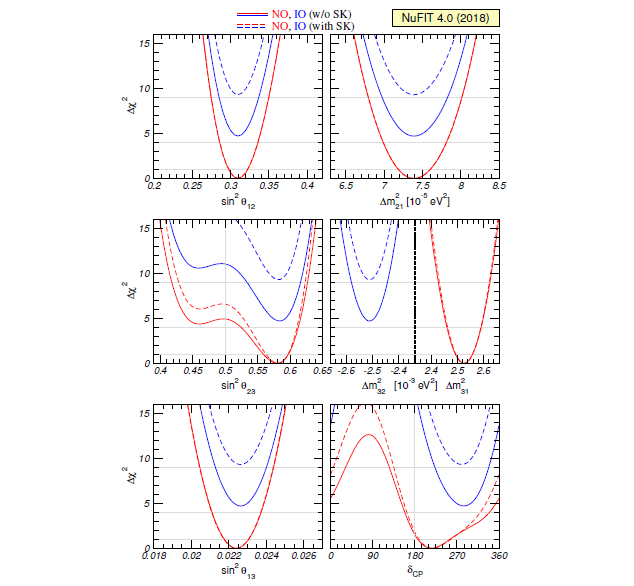
\includegraphics[width=0.87\textwidth]{massexp.png}
	\caption{\label{masshierarchy3:fig} $\Delta\chi^2$ profile obtained from global 3$\nu$ oscillation experiments analysis. The profiles are minimized in all non displayed parameters. The red and and blue full curves correspond to the analysis results for NO and IO respectively, without considering the atmospheric data from SuperK. The dashed lines are with the inclusion of this data. For atmospheric mass squared difference $\Delta m_{31}^2$ is used for NO and $\Delta m_{32}^2$ for IO. \cite{mass global fit}}
\end{figure}
\subsection {Mass hierarchy experimental results}
As already mentioned in Section \ref{sec: matter effects}, thanks to matter effects it is possible to study mass ordering in long baseline experiments by appearance measurements, typically $\nu_e$ appearance in $\nu_\mu$ beams. The most recent global fits performed on the oscillation parameters $\Delta m_{32}^2, \ \Delta m_{31}^2, \ \delta_{CP}$ and $\sin^2\theta_{23}$ from LBL accelerator experiments (NO$\nu$A, MINOS, T2K), reactor experiments (Data Bay, RENO, Double Chooz) and solar experiments (SNO, SuperK, Borexino) show a growing preference towards standard hierarchy. In particular the best fit can be obtained for NO while for IO one finds a $\Delta\chi ^2=4.7$ (Fig. \ref{masshierarchy3:fig}). The indication becomes even stronger when one includes data from the measurements on atmospheric neutrinos for SuperK where the value for IO becomes $\Delta\chi = 9.3$ \cite{mass global fit}.
\section{State of the art and future prospects}
\begin{figure}
	\centering
	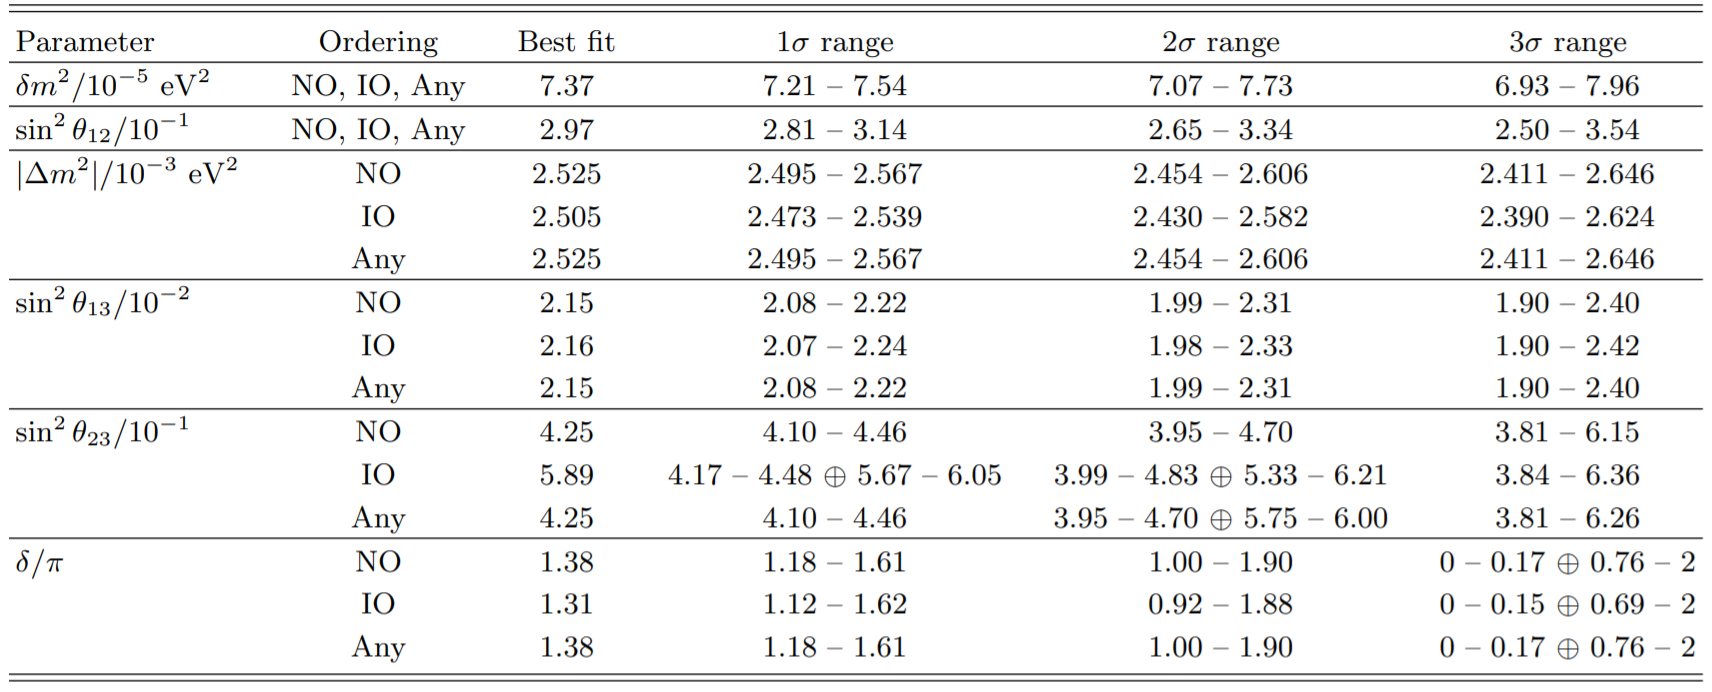
\includegraphics[width=1\textwidth]{stateoftheart.png}
	\caption{\label{stateof the art:fig} Results of recent $3\nu$ oscillation global fits. The results are given in terms of best fit and $n\sigma$ ranges under the IO, NO and any ordering assumptions. Note that here $\delta m^2 \equiv \Delta m_{12}^2$, $\Delta m^2 = m_3^2-(m_1^2+m_2^2)/2$ and $\delta \equiv \delta_{CP}$ is given in terms of cycle intervals $\delta/\pi \in [0,2]$. \cite{global constraints}} 
\end{figure}
Neutrino physics is entering its precision era with global fits restricting more and and more on the oscillation parameters values (Tab. \ref{stateof the art:fig}) \cite{global constraints}. As outlined in the previous sections though there are still fundamental questions that are yet to be fully answered : 
\begin{itemize}
	\item The determination of the absolute mass of the neutrinos and its origin i.e Majorana or Dirac;
	\item The measurement of CP asymmetries in the leptonic field;
	\item The determination of the mass ordering (normal or inverse)
\end{itemize}
While the first field of research is in the domain of the types of experiments described in Section and, the latter two are best studied in oscillation experiments. Such goals will require levels of precision still not achieved and new experiments in all categories (reactor, atmospheric, ecc.). \\
In the long-baseline accelerator field DUNE (Deep Underground Neutrino Experiment), will be the next-generation flagship neutrino oscillation experiment of the Fermilab national laboratories. Having access to MSW effects and to a neutrino beam capable of producing both $\nu_\mu$ and $\bar{\nu}_\mu$ will make it particularly well suited to probe mass hierarchy and CP violations respectively. This will be discussed more in detail in Chapter 2.


%%%%%%%%%%%%%%%%%%%%%%%%%%%%%%%%%%%%%%%%%%%%%%%%%%%%%%%%%%%%%%%%%%%%%%%%%%%%%

\chapter{DUNE}
The Deep Underground Neutrino Experiment (DUNE) will be a new generation world-leading Long Baseline oscillation experiment. Among its main goals are the precise measurement of the oscillation parameters, the study of matter-antimatter asymmetry and the determination of the neutrino mass ordering. It is conceived around three main components: The NuMi neutrino Beam, which is able to produce an intense and wide muon neutrino and antineutrino band; a fine-grained Near Detector (ND) situated at the Fermi National Accelerator Laboratories (Fermilab, Batavia, Illinois), just downstream of the neutrino source; a massive Liquid Argon Time Projection Chamber (LArTPC) Far Detector (FD) placed 1300 km downstream at the Sanford Underground Research Facility (Lead, South Dakota).\\
In this chapter we will discuss DUNE's physics programme (Section 1) as well as the configuration of the neutrino beam (Section 2) and its main detectors (Section 3). KLOE, which is one of DUNE's Near Detectors and the subject of the simulations performed for this thesis will be discussed more in detail in the next chapter.

\section{DUNE' s scientific program}

The scientific objectives of DUNE are categorized into a $primary$ and an $ancillary$ scientific programme. The latter is further divided into secondary objectives that could be persued by the experiment just by virtue of how it will be built and additional secondary objectives that may require specific upgrades to the facility.\\
The \emph{primary} programme is made up by the main measurements that DUNE will be built to perform with unprecedented precision which coincide with the fundamental questions that this experiment will try to answer:
\begin{enumerate}
	\item \textbf{Measurement of the charge-parity violating phase $\delta_{CP}$ and determination of the mass ordering of the neutrinos} (i.e. the sign of $\Delta m_{31}=m_3^2-m_1^2$). The study of $\delta_{CP}$ is particularly important in cosmological models trying to explain the matter-antimatter asymmetry in the universe.
	\item \textbf{Precision measurements of the $\nu_\mu \rightarrow \nu_{\mu,e}$ oscillation parameters}: the $\theta_{13}$ mixing angle; the $\theta_{23}$ mixing angle and the octant it lies in; the value of the $|\Delta m_{32}^2|$  mass difference. Precision measurements of these parameters and comparisons with corresponding patterns in the quark sector will further our knowledge of the underlying symmetries in fundamental particle physics.
	\item \textbf{Search for proton decay in one or more decay modes, improving significantly on previous lifetime limits}. Most Grand Unified Theories (GUTs) make lifetime predictions for nucleons and putting more and more stringent limits will be fundamental in assessing which one of them might be correct.
	\item \textbf{Detection and measurements of the neutrino flux from a core-collapse supernova}. In particular the time structure and energy spectrum of the neutrino burst would much further our understanding of this astrophysical phenomenon.
\end{enumerate}

The \emph{ancillary} programme consists of objectives that DUNE is not specifically conceived to achieve, but that are nonetheless enabled by the facility's design.:
\begin{enumerate}
	\item Further accelerator oscillation measurements and search for non-standard interactions beyond the standard model (BSD)
	\item Atmospheric neutrino oscillation measurements
	\item Measurements of other astrophysical phenomena using moderate energy neutrinos
\end{enumerate}
Finally the \emph{additional secondary} programme includes measurements potentially made possible by future upgrades to the facility such as monitoring of the diffuse supernova flux, solar neutrino and other low energy astrophysical neutrino measurements.\\
The high granularity and precision required by the \emph{DUNE Near Detector (ND)} will also allow it to have a scientific programme of its own. Its main objective will be to perform all the precision measurements necessary to acieve the goals of the primary programme. It will also pursue precision studies of the weak interaction, studies of nuclear and nucleon structure and searches for new physics.

\subsection{Sensitivities and systematics} 

In order to make any precision measurement one should be acutely aware of the systematic uncertainties related to the analysis strategy and the performance of the detector. In a two detectors Long Baseline experiment the $\nu_\mu$ spectrum measured in the Near Detector $N_{ND}^{data}(\nu_\mu)$ is propagated to the Far Detector and is used to predict the expected signal of $\nu_\mu$ and oscillated $\nu_e$ (and much smaller component of oscillated $\nu_\tau$) i.e. $N_{FD}^{exp}(\nu_\mu)$ and $N_{FD}^{exp}(\nu_e)$. Likewise the $\nu_e$ measured spectrum in the ND, mostly comprised of electron neutrinos from the beam and misidentified NC$\pi^0$ is used to predict the background at the FD. \\
The measured neutrino spectrum at the near detector is given by:
\begin{equation}
N_{ND}^{data}(\nu_{\mu,e})= \Phi_{ND}(\nu_{\mu,e}) \otimes \varepsilon_{ND}(\nu_{\mu,e}) \otimes \sigma_{ND}(\nu_{\mu,e})
\end{equation}
where $\Phi_{ND}(\nu_{\mu,e})$ is the beam flux, $\varepsilon_{ND}(\nu_{\mu,e})$ is the detector's efficiency and $\varepsilon_{ND}(\nu_{\mu,e})$ is the neutrino interaction cross section. In order to use such data to predict the signal and background expected at the far detector one needs to take into consideration:
\begin{itemize}
	\item \emph{Differences in how the neutrino interact $\sigma_{FD}/\sigma_{ND}$.} These are null in the case that the target nuclei in the Near and Far Detector are the same. Otherwise the dominating uncertainties in the prediction of $\nu_e$ in FD from measurement of $\nu_\mu$ in ND are the ones arising from differences in the electronic and muonic cross sections between the detectors: $\sigma_{FD}(\nu_e)/\sigma_{ND}(\nu_\mu)$.
	\item \emph{Differences in detector efficiencies $\varepsilon_{FD}/\varepsilon_{ND}$.} These uncertainties mostly arise from the differences in event selection between the two detectors and in particular the modelling of the energy scales. These are also virtually inexistent in the case that ND and FD are identical.
	\item \emph{Differences in the neutrino flux $\Phi_{FD}/\Phi_{ND}$.} The fluxes at the Near and Far detector are radically different since the ND is very close to the beamline and sees an expended source, while the FD is 1300 km away. A Monte Carlo is used to simulate the beam propagation, but it is itself not immune from inaccuracies: errors in the hadron production, focusing of the horns composition of the beam pipe and decay channel geometry can all contribute. 
\end{itemize} 
\begin{figure}
	\centering
	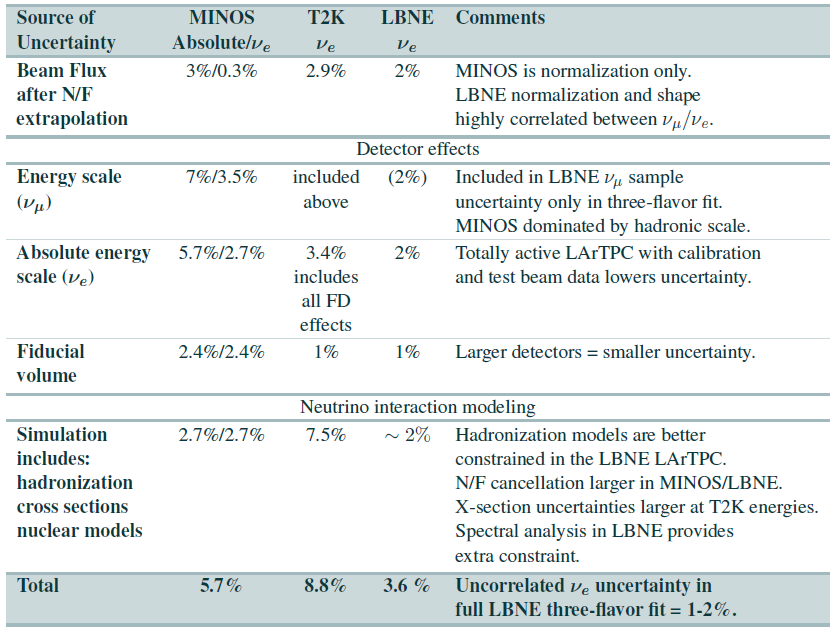
\includegraphics[width=0.81\textwidth]{uncertainties.png}
	\caption{\label{uncertainties:fig} Dominant systematics on the $\nu_e$ appearence channel for T2K and MINOS and projection for LBNE (Long Baseline Neutrino Experiment), the preliminary name used for DUNE} 
\end{figure}
Taking all of this into consideration one can then use neutrinos' oscillation and survival probability in order to predict the muonic and electronic signal in the Far Detector. The $\nu_\mu$ expected signal is given by:
\begin{equation}
N_{FD}^{exp}(\nu_\mu) = N_{ND}^{data}(\nu_\mu) \otimes \frac{\Phi_{FD}(\nu_\mu)}{\Phi_{ND}(\nu_\mu)} \otimes P(\nu_\mu \rightarrow \nu_\mu) \otimes \frac{\varepsilon_{FD}(\nu_\mu)}{\varepsilon_{ND}(\nu_\mu)} \otimes \frac{\sigma_{FD}(\nu_\mu)}{\sigma_{ND}(\nu_\mu)} 
\end{equation}
The $\nu_e$ expected signal is given by:
\begin{equation}
\begin{split}
N_{FD}^{exp}(\nu_\mu) & = \underbrace{N_{ND}^{data}(\nu_\mu) \otimes \frac{\Phi_{FD}(\nu_\mu)}{\Phi_{ND}(\nu_\mu)} \otimes P(\nu_\mu \rightarrow \nu_e) \otimes \frac{\varepsilon_{FD}(\nu_e)}{\varepsilon_{ND}(\nu_\mu)} \otimes \frac{\sigma_{FD}(\nu_e)}{\sigma_{ND}(\nu_\mu)}}_{\text{Expected signal}} \\
& + \underbrace{N_{ND}^{data}(\nu_e) \otimes \frac{\Phi_{FD}(\nu_e)}{\Phi_{ND}(\nu_e)} \otimes P(\nu_e \rightarrow \nu_e) \otimes \frac{\varepsilon_{FD}(\nu_e)}{\varepsilon_{ND}(\nu_e)} \otimes \frac{\sigma_{FD}(\nu_e)}{\sigma_{ND}(\nu_e)}}_{\text{Electronic events from the beam}} \\
& + \pi^0\text{NC background prediction from }N_{ND}^{data}(\nu_e)\\
& + \nu_\tau \text{ background prediction from }N_{ND}^{data}(\nu_\mu)
\end{split}
\end{equation}
The main sources of uncertainties are well known from previous experiments such as T2K and MINOS. They include:
\begin{itemize}
	\item \emph{Beam flux uncertainties}: related to the precision with which the ND is capable to measure the unoscillated beam flux in both shape and normalization.
	\item \emph{$\nu_\mu$ energy-scale uncertainties}: the muonic neutrino energy spectrum measured in the ND is then used to predict the $\nu_e$ appearance channel in the FD and the energy scale uncertainty scale is thus propagated.
	\item \emph{Absolute $\nu_e$ energy-scale uncertainty}: an accurate measurement of the shape of the $\nu_e$ appearance channel is essential to oscillation sensitivity and depends on how well the detector response is understood
	\item \emph{Simulation uncertainties}: uncertainties related to the modelling of the neutrino interactions with the target nuclei in the near and far detectors.
\end{itemize}
In Table \ref{uncertainties:fig} the dominant uncertainties for $\nu_e$ appearance for the T2K and MINOS and a preliminary prediction for DUNE are summarized. The precision is expected to improve from all fronts.



\subsection{Mass ordering and $\delta_{CP}$}
As it can be seen from Eq. \ref{eq:asymmetry} both a non-zero $\delta_{CP}$ and matter effects can induce asymmetries between $P(\nu_\mu \rightarrow \nu_e)$ and $P(\bar{\nu_\mu} \rightarrow \bar{\nu_e})$and thus:
\begin{equation}
\mathcal{A_{CP}}= \mathcal{A}_{\delta}+ \mathcal{A}_{matter}
\end{equation}
In figure \ref{oscillograms:fig} the asymmetries induced by CP violation ($\mathcal{A}_{\delta}$) in case that $\delta_{CP}=\pm\pi/2$ and by matter effects ($\mathcal{A}_{matter}$) are plotted separatly in 2d oscillograms as a function of baseline and Energy. In reality though the two asymmetries always operate at the same time if $\delta_{CP}$ is not null and the matter effects are not trivial. In experiments where both are relevant then, if one wants to use  measurements of total asymmetry both to measure $\delta_{CP}$ and the mass ordering, then it's mandatory to be able to disambiguate between the two. \\
For the MSW effects in particular the asymmetries are introduced by a CP violating term $P_{\sin\delta}$ in the oscillation probability:
\begin{equation}
P(\nu_\mu \rightarrow \nu_e) \simeq P(\nu_e \rightarrow \nu_\mu) \simeq P_0+P_{\sin\delta}+P_{\cos\delta}+P_3
\end{equation}
where
\begin{equation}
P_0=\sin^2\theta_{23}\frac{\sin^22\theta_{13}}{(A-1)^2}\sin^2[(A-1)\Delta]
\end{equation}
\begin{equation}
P_3=\alpha^2\cos^2\theta_{13}\frac{\sin^22\theta_{12}}{A^2}\sin^2(A\Delta)
\end{equation}
\begin{equation}
P_{\sin\delta}=\alpha\frac{8J_{CP}}{A(1-A)}\sin\Delta\sin(\Delta A)\sin((1-A)\Delta)
\end{equation}
\begin{equation}
P_{\cos\delta}=\alpha\frac{8J_{CP}\cot \delta_{CP}}{A(1-A)}\sin\Delta\sin(\Delta A)\sin((1-A)\Delta)
\end{equation}
with 
\begin{equation}
\Delta = \Delta m_{31}^2 L/4E
\end{equation}
\begin{equation}
A=\sqrt{3}G_FN_e2E/\Delta m_{31}^2
\end{equation} 
\begin{equation}
\alpha = |\Delta m_{12}^2 |/|\Delta m_{31}^2 |
\end{equation}
\\
Note that since the value of $\Delta m_{31}^2$ switches between normal and inverted hierarchy, the asymmetry effects induced by the passage through matter will also be different: for normal (inverted) hierarchy $P(\nu_\mu-\nu_e)$ is enhanced (suppressed) and $P(\bar{\nu_\mu}-\bar{\nu_e})$ is suppressed (enhanced); 
the matter effects shift the phase of oscillation pattern for a fixed baseline to lower energies (by about -100 MeV) in the IH. \\
In general the matter effects have the largest impacts when the oscillation nodes for $\theta_{13}$ are reached (the first two nodes are highlighted in black in Fig. \ref{oscillograms:fig}):
\begin{equation}
\frac{L(\text{km})}{E(\text{GeV})} = (2n-1)\frac{\pi}{2}\frac{1}{(1.27\times\Delta m_{31}^2(\text{eV}^2))} \simeq(2n-1)\times 510 \text{km/GeV}
\end{equation}
For an experiment such as DUNE, where we have a baseline of $L\sim1300$km (highlighted in black in Fig. \ref{oscillograms:fig}) and an energy range $E\sim5-10$ GeV, the matter effects are maximal, and it is then crucial that they are disentangled from the CP effects.\\
Knowing the value of $|\Delta m_{31}^2 |$ (only the sign is still unknown), one can see, though, that for a baseline $>$1200km, the size of $\mathcal{A}_{matter}$ surpasses the highest possible value of $\mathcal{A}_{\delta}$ which makes the disambiguation between the two effects possible. In Figure the plots show the total asymmetry at the first (black) and second (red) as a function of $\delta_{CP}$ for four different values of $L$: 290km,810km,1300km (baseline of DUNE) and 2300km. The NH and IH the total asymmetries will have different values because of the matter effects and are plotted as full and dashed lines respectively. As the baseline gets bigger, given the same node, the CP-induced asymmetry will stay the same while matter induced one will get bigger since the dependencies on $L$ and E are:
\begin{equation}
\mathcal{A}_{\delta} \propto L/E
\end{equation}
\begin{equation}
\mathcal{A}_{matter} \propto L\times E
\end{equation}
If one considers then the case in which the $\delta_{CP}$ asymmetries is maximal (green line in the plots) is easy to see that if $\mathcal{A}_{matter} < \mathcal{A}_\delta(max)$ the same total asymmetry is compatible with both hierarchies and multiple value of $\delta_{CP}$. This is true for baselines shorter than 1200km. For DUNE, where $L\sim1300$km these ambiguities don't exist.
\begin{figure}
	\centering
	\includegraphics[width=0.85\textwidth]{oscillograms.png}
	\caption{\label{oscillograms:fig} $\mathcal{A}_{CP}$ total asymmetry as a function of baseline and energy. The top two oscillograms show the asymmetry for $\delta_{CP}=0$ (i.e. $\mathcal{A}_{matter}$) for Normal(left) and Inverted (right) mass ordering. The two bottom oscillograms show the asymmetry in vacuum (i.e. $\mathcal{A}_{\delta}$) for $\delta_CP=\pi/2$ (left) and $\delta_CP=-\pi/2$ (right). DUNE's baseline (1300km) and the 1st and 2nd oscillation nodes are highlighted in black.  } 
\end{figure}
\subsubsection{Significance for mass ordering and $\delta_{CP}$ measurements}
\begin{figure}
	\centering
	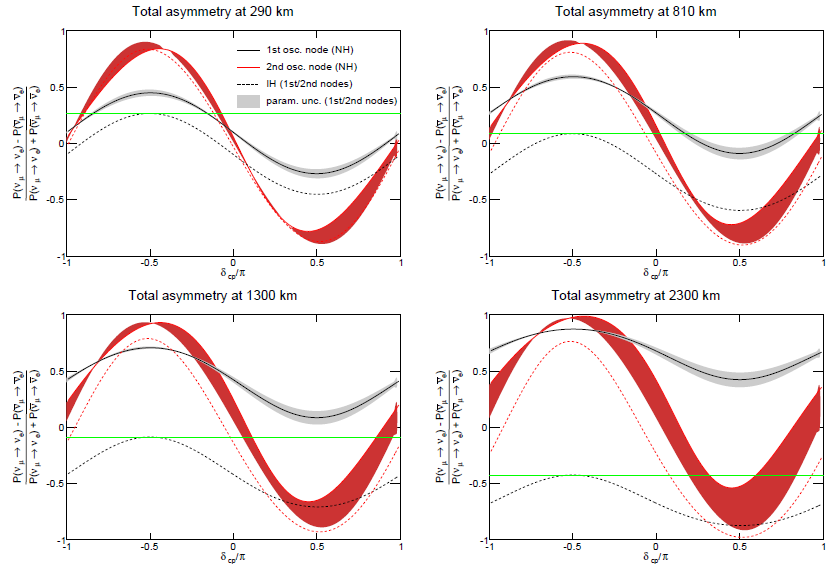
\includegraphics[width=0.8\textwidth]{asymmetrydelta.png}
	\caption{\label{asymmetrydelta:fig} Total $\mathcal{A}_{CP}$ as a function of $\delta_{CP}/\pi$ for four different baselines (290km, 810km, 1300km and 2300km). The black (red) lines indicate the asymmetries at the first (second) node, the full ones being for NH and the dashed ones for IH. } 
\end{figure}
The sensitivity with which the DUNE experiment will be able to measure the mass ordering (MO) and CP-Violation (CPV), is evaluated by fitting the simulated oscillation spectra of $\nu_\mu \rightarrow \nu_{\mu,e}$ and $\bar{\nu}_\mu \rightarrow \bar{\nu}_{\mu,e}$ for different values of the oscillation parameters and confronting the results with the expected "true" theoretical values in terms of $\Delta\chi^2$:
\begin{equation}
\Delta\chi^2_{MO}= |\chi^2_{MH^{test}=IH}-\chi^2_{MH^{test}=NH}| 
\end{equation}
\begin{equation}
\Delta\chi^2_{CPV}= \min (\Delta\chi^2_{CP}(\delta_{CP}^{test}=0),\Delta\chi^2_{CP}(\delta_{CP}^{test}=\pi))
\end{equation}
with $\Delta\chi^2_{CP}=\chi^2(\delta_{CP}^{test})-\chi^2(\delta_{CP}^{true})$. The significance with which DUNE will be able to assess the mass ordering grows with the exposure , defined as kt of active volume $\times$ MW beam?s power $\times$ years, and varies wildly with the value of $\delta_{CP}$ (Fig.\ref{exposure-MO:fig}). In order to ensure the DUNE objective of reaching $\sqrt{\Delta\chi^2}=5$ for every value of $\delta_{CP}$ approximately an exposure of 200-400 kt$\times$MW$\times$years will be need. The significance for $\delta_{CP}$ similarly grows with exposure (Fig.\ref{exposure-deltaCP:fig}), but only for values different from 0 and $\pi$, for which there is no CP violation and $\sqrt{\Delta\chi^2}=0$ always. The significance for both MO and CPV also depends strongly on the values of all the oscillation parameters (Fig. \ref{MOsignificance-param:fig} and  \ref{CPVsignificance-param:fig}), making precision measurements with DUNE mandatory.
\begin{figure}
	\centering
	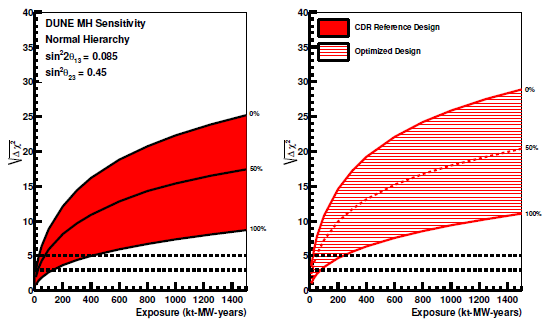
\includegraphics[width=0.7\textwidth]{exposure-MO.png}
	\caption{\label{exposure-MO:fig} MO significance as a function of exposure for two different beam designs (left and right) and three values of CP asymmetry (0\%,50\%,100\%).  } 
\end{figure}
\begin{figure}
	\centering
	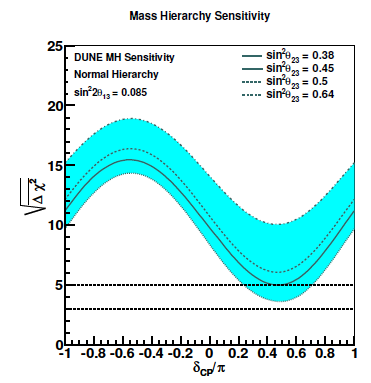
\includegraphics[width=0.375\textwidth]{MOVStheta23.png}
	\qquad
	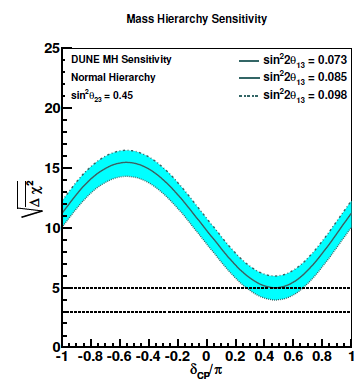
\includegraphics[width=0.375\textwidth]{MOVStheta13.png}
	\qquad
	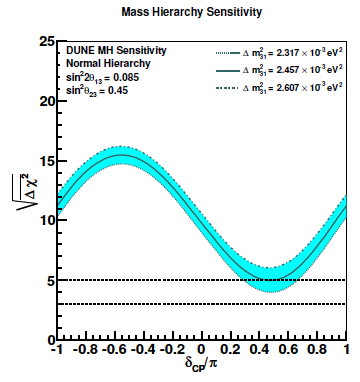
\includegraphics[width=0.375\textwidth]{MOVSm31.png}
	\caption{\label{MOsignificance-param:fig} MO significance as a function of $\delta_{CP}/\pi$ at a fix value of exposure 300 kt$\times$MW$\times$years for different values of the oscillation parameters: $\theta_23$ (upper-left), $\theta_13$ (upper-right), $\delta m_{31}^2$ (bottom)} 
\end{figure}

\begin{figure}
	\centering
	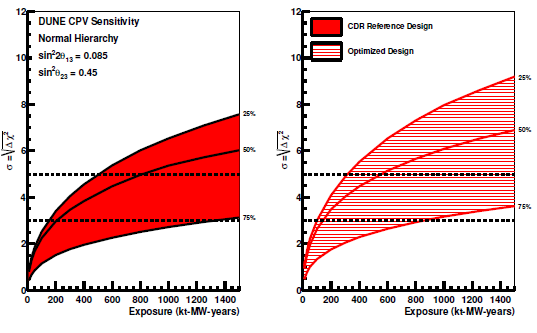
\includegraphics[width=0.7\textwidth]{exposure-CPV.png}
	\caption{\label{exposure-deltaCP:fig} CPV significance as a function of exposure for two different beam designs (left and right) and three values of CP asymmetry (0\%,50\%,100\%).  } 
\end{figure}
\begin{figure}
	\centering
	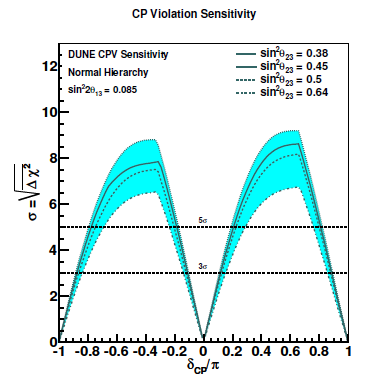
\includegraphics[width=0.375\textwidth]{CPVVStheta23.png}
	\qquad
	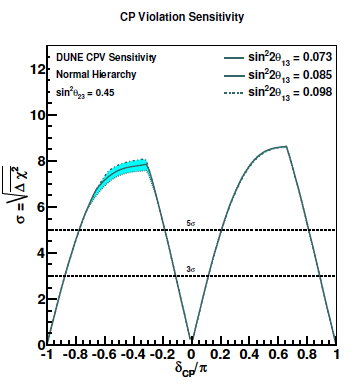
\includegraphics[width=0.375\textwidth]{CPVVStheta13.png}
	\qquad
	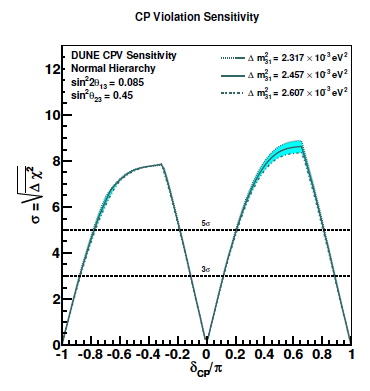
\includegraphics[width=0.375\textwidth]{CPVVSm31.png}
	\caption{\label{CPVsignificance-param:fig} CPV significance as a function of $\delta_{CP}/\pi$ at a fix value of exposure 300 kt$\times$MW$\times$years for different values of the oscillation parameters: $\theta_23$ (upper-left), $\theta_13$ (upper-right), $\delta m_{31}^2$ (bottom)} 
\end{figure}
\subsection{Precision Mesurements}
\begin{figure}
	\centering
	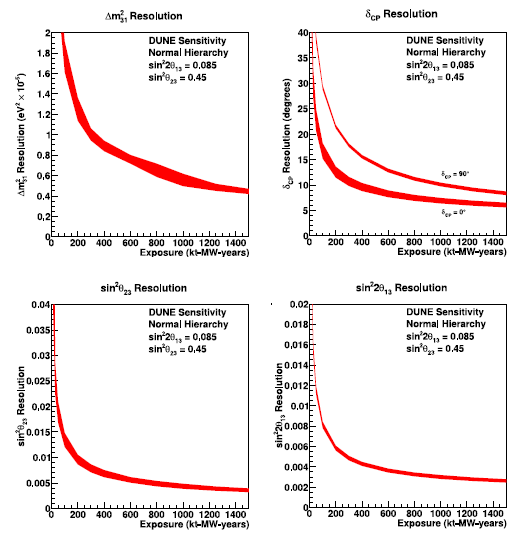
\includegraphics[width=0.75\textwidth]{precision.png}
	\caption{\label{precision:fig} Resolution as a function of exposure for $\Delta m_{31}^2$ (upper left), $\delta_{CP}$ (upper right), $\sin^\theta_{23}$ (bottom left) and $\sin^2\theta_{13}$ (bottom right). The red area represents the range in sensitivity du to differences in beam design.  } 
\end{figure}
The DUNE experiment will improve sensitivity on the key parameters governing $\nu_1-\nu_2$ and $\nu_2-\nu_3$: 
\begin{itemize}
	\item $\sin^2\theta_{23}$ and the octant of $\theta_{23}$;
	\item$\delta_{P}$; \item$\sin^2\theta_{13}$;
	\item$\Delta m_{31}^2$.
\end{itemize}
The sensitivity to these parameters as a function of exposure is plotted in Figure \ref{precision:fig} \\
Determining the octant of the mixing angle $\theta_{23}$, and thus if its value is exactly $45^\circ$ producing maximal mixing between mass eigenstates 2 and 3 $\sin^2\theta_{23}$ is still an open question, with the latest results from T2K leaving both a lower ($<45^\circ$) and upper ($<45^\circ$) octant scenarios open, depending on the mass hierarchy being considered. This particular question is of great theoretical interest. A value of $\theta_{23}$ being exactly $45^\circ$ would hint at new nt yet considered symmetries, while for example an excess in the upper octant of the order of the Cabibbo angle, point in the direction of quark-lepton universality models. \\
The measurement of the octant is made possible by combining survival ($\nu_\mu \rightarrow \nu_\mu$) and oscillation($\nu_\mu \rightarrow \nu_e$) probabilities, the firt being sensitiveto $\sin^22\theta_{23}$ an the second to  $\sin^2\theta_{23}$. The $\Delta\chi^2$ for the determination of th octant is then:
\begin{equation}
\Delta\chi^2_{octant}=|\chi^2_{\theta_{23}>45^\circ}- \chi^2_{\theta_{23}<45^\circ}|
\end{equation}
The sensitivity to the octant as a function of $\theta_{23}$ is plotted in Fig.\ref{octant:fig}\\
DUNE will also be able to perform unitarity tests of the PMNS matrix by measuring precisely the value of $\sin2\theta_{13}$, which will constrain the phase space of possible new physics. In general th high precision measurement performed by dune could reveal new physics driven for example by non-standard interactions or the existence sterile neutrinos.
\begin{figure}
	\centering
	\includegraphics[width=0.6\textwidth]{octant.png}
	\caption{\label{octant:fig} $\Delta\chi^2_{octant}$ as a function of $\theta_{23}$. Th yellow areas indicate the $1\sigma$ and $3\sigma$ intervals for the value of $\theta_{23}$ from recent global fits. The green area represents the range in sensitivity due to differences is beam design and $\delta_{CP}$ value.} 
\end{figure}  
\subsection{Oscillation physics with atmospheric neutrinos}
\begin{thebibliography}{90}             %crea l'ambiente bibliografia
\rhead[\fancyplain{}{\bfseries \leftmark}]{\fancyplain{}{\bfseries
\thepage}}
%%%%%%%%%%%%%%%%%%%%%%%%%%%%%%%%%%%%%%%%%aggiunge la voce Bibliografia
                                        %   nell'indice
\addcontentsline{toc}{chapter}{Bibliografia}
%%%%%%%%%%%%%%%%%%%%%%%%%%%%%%%%%%%%%%%%%provare anche questo comando:
%%%%%%%%%%%\addcontentsline{toc}{chapter}{\numberline{}{Bibliografia}}
\bibitem{Pauli} W. Pauli, "Letter to a physicist's gathering at Tubingen", December 4,
1930. Reprinted in Wolfgang Pauli, Collected Scientific Papers, ed. R.
Kronig and V. Weisskopf, Vol. 2, p. 1313 (Interscience: New York, 1964).
\bibitem{Fermi} E. Fermi, "Tentativo di una Teoria Dei Raggi $\beta$", Il Nuovo Cimento, vol. 11, pp. 1-19, Jan 1934
\bibitem{Bethe-Peierls} H. Bethe and R.Peierls, "The neutrino", Nature, vol.133, p.532, 1934
\bibitem{Pontecorvo} B. Pontecorvo, "Inverse beta process" Camb. Monogr. Part. Phys. Nucl. Phys. Cosmol.,
vol. 1, pp. 25?31, 1991.
\bibitem{Reines-Cowan}F. Reines and C. L. Cowan, "The neutrino" Nature, vol. 178, pp. 446?449, Sep 1956.
\bibitem{Lederman-Misty-Steinberg}G. Danby, J. M. Gaillard, K. A. Goulianos, L. M. Lederman, N. B. Mistry, M. Schwartz, and
J. Steinberger, "Observation of High-Energy Neutrino Reactions and the Existence of Two Kinds
of Neutrinos", Phys. Rev. Lett., vol. 9, pp. 36?44, 1962.
\bibitem {LEP} ALEPH Collaboration, D. Decamp et al., Phys. Lett. B 235, pp.399, 1990
\bibitem{DONUT} DONUT Collaboration, K. Kodama et al., Phys. Lett. B 504,
pp. 218-224, 2001.
\bibitem{Lipari} P. Lipari, "Introduction to neutrino physics", chapter 13:"Models for neutrino masses" in 2001 CERN-CLAF School of high-energy
physics, Itacuruca, Brazil, 6-19 May, 2001: Proceedings, pp. 115?199, 2001.
\bibitem{Petcov} S. T. Petcov, "The Nature of Massive Neutrinos", Adv. High Energy Phys., vol. 2013,
p. 852987, 2013.
\bibitem{Troisk}V. N. Aseev et al., "An upper limit on electron antineutrino mass from Troitsk
experiment", Phys. Rev., vol. D84, p. 112003, 2011
\bibitem{Mainz}C. Kraus et al., "Final results from phase II of the Mainz neutrino mass search in
tritium beta decay", Eur. Phys. J., vol. C40, pp. 447?468, 2005.
\bibitem{KATRIN} Aker 2019, "Improved Upper Limit on the Neutrino Mass from a Direct Kinematic Method by KATRIN",123, 1079-7114, Physical Review Letters, American Physical Society (APS), Aker, M. and Altenm�ller, K. and Arenz, M. and Babutzka, M. and Barrett, J. and Bauer, S. and Beck, M. and Beglarian, A. and Behrens, J. and Bergmann, T. and et al. 2019 Nov
\bibitem{PDG} M. Tanabashi et al., "Review of particle physics", Phys. Rev. D, vol. 98, p. 030001,
Aug 2018.
\bibitem {Zuber} K. Zuber, Neutrino Physics, Second Edition. Aug. 2011.
\bibitem{Giunti} C. Giunti and C. W. Kim, Fundamentals of Neutrino Physics and Astrophysics.
2007.
\bibitem {Wolfenstein} L. Wolfenstein, Phys. Rev. D17 (1978) 2369; S.P. Mikhaev and A.Y.
Smirnov, Sov.J.Nucl.Phys. 42 (1985) 913; S.P. Mikhaev and A.Y.
Smirnov, Nuovo Cimento C9 (1986) 17.
\bibitem{Ricciardi} Stefania Ricciardi, "Lecture notes on Neutrino oscillations in matter", 6/10/2013
\bibitem{Bahcall} J. N. Bahcall, M. H. Pinsonneault, and S. Basu, "Solar models: Current epoch and time dependences,
neutrinos, and helioseismological properties", Astrophys. J., vol. 555, pp. 990?1012, 2001,
\bibitem{Homestake} K. Lande and P. Wildenhain, "The homestake chlorine solar neutrino experiment?past,
present and future", Nuclear Physics B - Proceedings Supplements, vol. 118, pp. 49?54,
Apr 2003.
\bibitem{Gallex} J. N. Abdurashitov, E. P. Veretenkin, V. M. Vermul, V. N. Gavrin, S. V. Girin, V. V.
Gorbachev, P. P. Gurkina, G. T. Zatsepin, T. V. Ibragimova, A. V. Kalikhov, and et al.,
"Solar neutrino flux measurements by the soviet-american gallium experiment (sage) for
half the 22-year solar cycle", Journal of Experimental and Theoretical Physics, vol. 95,
pp. 181?193, Aug 2002.
\bibitem{Sage} M. Altmann and Others, "Complete results for five years of gno solar neutrino observations",
Physics Letters B, vol. 616, no. 3, pp. 174 ? 190, 2005.
\bibitem {SuperK} Y. Suzuki, "The super-kamiokande experiment", The European Physical Journal C,
vol. 79, Apr 2019.
\bibitem{SNO} Q. R. Ahmad et al., "Direct evidence for neutrino flavor transformation from neutral current interactions
in the Sudbury Neutrino Observatory", Phys. Rev. Lett., vol. 89, p. 011301, 2002, nuclex/
0204008.
\bibitem{kamland} S. Abe, T. Ebihara, S. Enomoto, K. Furuno, Y. Gando, K. Ichimura, H. Ikeda, K. Inoue,
Y. Kibe, Y. Kishimoto, and et al., "Precision measurement of neutrino oscillation
parameters with kamland",Physical Review Letters, vol. 100, Jun 2008.
\bibitem{Borexino} G. Alimonti and Others, "The borexino detector at the laboratori nazionali del gran
sasso", Nuclear Instruments and Methods in Physics Research Section A: Accelerators,
Spectrometers, Detectors and Associated Equipment, vol. 600, pp. 568?593, Mar 2009.
\bibitem{Wagner} Valle, Jos� Wagner Furtado, and Jorge Romao. "Neutrinos in High Energy and Astroparticle Physics"", John Wiley \& Sons, Incorporated, 2055
\bibitem{Data Bay} F. An and Others, "Measurement of electron antineutrino oscillation based on 1230 days
of operation of the daya bay experiment", Physical Review D, vol. 95, Apr 2017
\bibitem{RENO} S.-B. Kim, "New results from reno and prospects with reno-50", Nuclear and Particle
Physics Proceedings, vol. 265-266, pp. 93?98, Aug 2015.
\bibitem{Double Chooz} J. I. Crespo-Anad�n, "Double Chooz: Latest results," Nucl. Part. Phys. Proc., vol. 265-
266, pp. 99?104, 2015.
\bibitem{Farzan-Tortola}Y. Farzan and M. Tortola, "Neutrino oscillations and Non-Standard Interactions",
Front.in Phys., vol. 6, p. 10, 2018.
\bibitem{Superk atm}Y. Ashie et al., "A Measurement of atmospheric neutrino oscillation parameters by SUPERKAMIOKANDE
I," Phys. Rev., vol. D71, p. 112005, 2005, hep-ex/0501064.
\bibitem{soudan 2} W. W. M. Allison et al., "Measurement of the atmospheric neutrino flavor composition
in Soudan-2", Phys. Lett., vol. B391, pp. 491?500, 1997.
\bibitem{MACRO} G. Giacomelli, "Neutrino physics and astrophysics with the MACRO experiment at the
Gran Sasso lab", Braz. J. Phys., vol. 33, pp. 211?217, 2003.
\bibitem{k2k} S. Boyd, "Recent results from the k2k (kek-to-kamioka) neutrino oscillation experiment",
Nuclear Physics B - Proceedings Supplements, vol. 98, pp. 175?181, Apr 2001.
\bibitem{MINOS} J. Evans, "The MINOS Experiment: Results and Prospects", Adv. High Energy Phys., vol. 2013, p. 182537, 2013.
\bibitem {OPERA} N. Agafonova, A. Alexandrov, A. Anokhina, S. Aoki, A. Ariga, T. Ariga, A. Bertolin,
C. Bozza, R. Brugnera, A. Buonaura, and et al., "Final Results of the OPERA Experiment
on $\nu_\tau$ Appearance in the CNGS Neutrino Beam", Physical Review Letters, vol. 120, May 2018.
\bibitem{Nomad} F. Vannucci, "The nomad experiment at cern", Advances in High Energy Physics,
vol. 2014, pp. 1?20, 2014.
\bibitem{Chorus} A. G. Cocco, "Results from CHORUS experiment at CERN," Phys. Rept., vol. 307,
pp. 319?324, 1998.
\bibitem{T2K} C. Giganti, "Latest results from T2K and T2K Phase II," in Proceedings, Prospects in Neutrino Physics (NuPhys2017): London, UK, December 20-22, 2017, pp. 61?69, 2018.
\bibitem{Nova} F. Jediny, "Nova latest results", Proceedings of The 15th International Conference on
Flavor Physics \& CP Violation ? PoS(FPCP2017), Oct 2017.
\bibitem{deltaCP} W. Marciano and Z. Parsa, "Intense neutrino beams and leptonic CP violation",
Nucl. Phys. Proc. Suppl., vol. 221, pp. 166?172, 2011.
\bibitem{t2k deltacp} K. Abe et al., "Measurement of neutrino and antineutrino oscillations by the t2k
experiment including a new additional sample of $\nu_e$ interactions at the far detector",
Phys. Rev. D, vol. 96, p. 092006, Nov 2017.
\bibitem{mass global fit}I. Esteban, M. C. Gonzalez-Garcia, A. Hernandez-Cabezudo, M. Maltoni, and
T. Schwetz, "Global analysis of three-flavour neutrino oscillations: synergies and
tensions in the determination of $\theta_{23}$; $\delta_{CP}$, and the mass ordering", JHEP, vol. 01,
p. 106, 2019
\bibitem{global constraints} F. Capozzi, E. Di Valentino, E. Lisi, A. Marrone, A. Melchiorri, and A. Palazzo,
"Global constraints on absolute neutrino masses and their ordering", Phys. Rev.,
vol. D95, no. 9, p. 096014, 2017.
\end{thebibliography}
%%%%%%%%%%%%%%%%%%%%%%%%%%%%%%%%%%%%%%%%%non numera l'ultima pagina sinistra

\end{document}